% GeoPRR-Net manuscript prepared with the repository's official MDPI class.
% Main file for Overleaf: manuscript.tex

\documentclass[electronics,article,submit,oneauthor]{Definitions/mdpi}

% Publisher-only DOI and submission-date marks are intentionally hidden in the
% author manuscript. MDPI assigns these metadata during production. Set this
% switch to true only if the editorial office requests the production footer.
\newif\ifmdpipublishermetadata
\mdpipublishermetadatafalse
\makeatletter
\AtBeginDocument{%
  \ifmdpipublishermetadata\else
    \fancypagestyle{plain}{%
      \fancyhf{}%
      \fancyfoot[C]{\footnotesize\thepage}%
      \renewcommand{\headrulewidth}{0pt}%
      \renewcommand{\footrulewidth}{0pt}}%
    \pagestyle{fancy}%
    \fancyhf{}%
    \fancyfoot[C]{\footnotesize\thepage}%
    \renewcommand{\headrulewidth}{0pt}%
    \renewcommand{\footrulewidth}{0pt}%
  \fi
}
\makeatother

%=================================================================
% MDPI metadata
\firstpage{1}
\makeatletter
\setcounter{page}{\@firstpage}
\makeatother
\pubvolume{1}
\issuenum{1}
\articlenumber{0}
\pubyear{2026}
\copyrightyear{2026}
\datereceived{}
\daterevised{}
\dateaccepted{}
\datepublished{}

%=================================================================
% Local commands
\usepackage{xspace}
\newcommand{\modelname}{GeoPRR-Net\xspace}
\newcommand{\nmae}{\mathrm{NMAE}}
\graphicspath{{figures/}}

%=================================================================
% Front matter. The provisional UCL affiliation must be confirmed with the
% institution or supervisor before submission.
\Title{\modelname: A Geometry-Aware Mixture of Heterogeneous Experts for Robust Analog Gauge Reading}

\Author{Xiaoyi Liang $^{1,*}$}
\AuthorNames{Xiaoyi Liang}

\address{$^{1}$ \quad University College London, London WC1E 6BT, United Kingdom; ucabx23@ucl.ac.uk}
\corres{Correspondence: ucabx23@ucl.ac.uk}

\abstract{Analog gauges remain common in legacy infrastructure, but blur and oblique viewpoints change the reliability of visual evidence. We present \modelname, a geometry-aware dense mixture of experts for normalized progress estimation. A shared EfficientNet-B0 processes raw and support-normalized observations. Geometry-aware fusion and relational moment transport produce complementary estimates, while an auxiliary polar branch supplies angular evidence. A conditional router combines their means, and an information projection expresses the routed estimate as one moment-consistent 128-bin posterior. On the official 4,000-image SyncG test split under six conditions, three source-seed fits achieve $0.7407\pm0.0220$\%FS NMAE, compared with $1.6595\pm0.0627$\%FS for the strongest tested raw CNN. Across source-training configurations, the retained no-geometry, fixed-mixture, and no-relational variants have NMAE 0.6045, 0.2697, and 0.1803\%FS above the updated full-model reference, respectively. Frozen transfer achieves $11.6235\pm1.6030$\%FS on Industrial-1395, a 15.1\% reduction relative to Raw EfficientNet-B0. In the retained original-configuration experiment with matched supervised group-wise out-of-fold adaptation, the reduction is 18.9\%, or 19.3\% when both methods use three-member equal-weight ensembles. These results support geometry-aware evidence fusion and conditional allocation for robust ROI-level gauge reading.}

\keyword{analog gauge reading; pointer meter reading; industrial vision; mixture of experts; conditional routing; projective distortion; polar representation; moment projection}

%%%%%%%%%%%%%%%%%%%%%%%%%%%%%%%%%%%%%%%%%%
\begin{document}

\section{Introduction}
\label{sec:introduction}

Analog gauges, also called pointer meters or analog pointer instruments, remain the last-mile interface to pressure, temperature, flow, and electrical state in substations, process plants, laboratories, and legacy equipment. Their operational relevance is visible in current safety requirements: U.S. occupational-safety rules still require every air receiver to carry an indicating pressure gauge that is readily visible, while the process-safety standard explicitly places monitoring devices, sensors, alarms, and interlocks within equipment subject to inspection and testing \cite{osha1910airreceivers,osha1910psm}. The visual reading interface is therefore not a historical curiosity; it remains embedded in active safety and maintenance practice.

Many installations predate networked sensing and cannot be replaced without shutdown, recertification, or substantial retrofit cost. Manual rounds are episodic and labor intensive, while delayed or incorrect transcription can hide a developing threshold event. Recent research consequently places camera readers on mobile and legged robots, in unstructured plants, and along automated substation inspection routes \cite{howells2021analogue,dong2021vdn,milana2022gauges,reitsma2024underpressure,chu2025prikmet}. Camera-based reading is valuable because it can turn an installed visual instrument into a remotely observable asset without altering the measurement chain.

The field problem is substantially harder than recognizing a clean, centered dial. A pointer may occupy only a few pixels in width, so motion or defocus blur can erase its boundary before the dial layout disappears. An oblique retrofit viewpoint changes a circular dial into a projective shape, and an imperfect ROI shifts the apparent relation among center, pointer, and scale. The practical cost of viewpoint is measurable: GAUREAD reported error within 3\% below a $20^{\circ}$ perspective angle but within 9\% at angles up to $50^{\circ}$ \cite{milana2022gauges}. These degradations do not reduce every cue uniformly; they change which representation deserves trust. Frontal images reward local geometry, blur favors more global structure, and projective views make raw image coordinates unreliable while cross-view relations can remain informative (Figure~\ref{fig:architecture}a).

Rectification, polar unwrapping, pointer segmentation, vector estimation, keypoint pose, and scale-mark geometry all provide useful structure for gauge reading \cite{bao2019ipm,li2020text,wu2021lowlight,dong2021vdn,wang2022scalemark,tan2024transunet}. Most readers, however, commit to one transformation or evidence path before the reliability of that path is known for the current image. The unresolved problem is therefore not simply how to add another representation, but how to arbitrate among complementary physical evidence while returning one coherent reading distribution.

Mixture-of-experts (MoE) models provide a natural language for this problem: specialized functions produce candidate outputs and an input-dependent gate determines their contribution \cite{jacobs1991adaptive}. Sparse and soft MoEs have demonstrated that routing can organize specialized capacity in both language and vision models \cite{shazeer2017sparsely,riquelme2021vmoe,puigcerver2024softmoe}. We adapt this principle to analog-gauge reading as a compact dense MoE: geometry/base, polar, and relational experts share one encoder, while the gate reweights their evidence according to observed geometry and representation quality.

We formulate that question as normalized single-pointer progress within known scale endpoints. This is a reusable industrial core because instrument ranges are often available from asset metadata, and a physical reading follows directly from an affine mapping. Separating progress estimation from OCR and range discovery isolates the difficult visual inference problem and permits matched ROI-level comparisons with standard CNN regressors, pointer-segmentation components, vector estimators, and keypoint-pose readers.

Evaluation must also reflect the value of field evidence. Synthetic data and SyncG provide exact labels and controlled stress tests \cite{howells2021analogue,leonalcazar2024synthetic,deng2026syncg}, but they cannot replace photographs acquired in working environments. Industrial-1395 consolidates 1,395 labeled real-instrument ROIs from three field-photo collections and 52 acquisition groups. Complete-cohort group-wise evaluation tests input-dependent expert mixing across the uncontrolled appearance, capture, and instrument variation that motivates the work in the first place.

We propose the Geometry-Aware Polar--Relational Routing Network (\modelname), organized as a dense mixture of heterogeneous evidence experts. A support-aware pixel operation constructs raw and conservatively normalized observations, which are processed by one shared EfficientNet-B0 encoder \cite{tan2019efficientnet}. Its feature hierarchy supports three experts: (i) a geometry-aware base expert built from aligned dual-view relations, (ii) a polar expert based on radial moments and a learned angular posterior, and (iii) a relational expert that transports the base moment using raw/normalized context differences. A conditional router, acting as the MoE gating network, places their candidate means on a convex simplex. Instead of averaging incompatible posterior shapes, the routed scalar target is imposed on the base distribution through one exponential information projection \cite{csiszar1975idivergence}. The output therefore remains a single 128-bin posterior with an exactly controlled first moment.

The study makes four contributions:
\begin{enumerate}[leftmargin=*]
    \item We formulate ROI-level gauge reading through shared representations of raw and support-normalized observations, retaining image-derived geometry and view availability as explicit evidence.
    \item We combine geometry-aware fusion and relational moment transport with conditional allocation of candidate means. A moment-consistent information projection returns one posterior whose mean agrees with the routed reading.
    \item We compare the updated full model with retained geometry, relational, and routing variants, including a geometry-by-routing comparison across source-training configurations.
    \item We compare three raw CNNs and three structured readers with \modelname on the official SyncG test split, followed by frozen transfer to RF100-VL and Industrial-1395. A separate matched OOF protocol gives the same target-domain supervision and ensemble size to the learned-feature baselines.
\end{enumerate}

The remainder of the paper is organized as follows. Section~\ref{sec:related} reviews related approaches. Section~\ref{sec:methods} defines the model and fitting procedure, and Section~\ref{sec:protocol} specifies the evaluation protocols. Section~\ref{sec:results} presents SyncG results, zero-shot transfer, matched field adaptation, the principal structural ablations, and complete-reader efficiency. Sections~\ref{sec:discussion} and~\ref{sec:conclusion} discuss the evidence and conclude the study.

\section{Related Work}
\label{sec:related}

\subsection{Geometric Correction and Staged Reading Pipelines}

Classical and hybrid gauge readers often make camera geometry explicit before estimating a pointer angle. Bao et al. used inverse perspective mapping with calibrated geometric references \cite{bao2019ipm}. Wu et al. combined mask-based perspective correction with pointer-direction regression for low-light scenes \cite{wu2021lowlight}. Scale-mark extraction and principal-axis geometry have also been used to recover the center and read gauges under illumination and perspective changes \cite{wang2022scalemark}. Such methods are interpretable, but their accuracy can depend on complete contours, calibration patterns, or reliable mark extraction.

Deep staged pipelines replace individual hand-engineered components without eliminating the sequence. Sun et al. organized detection, segmentation, OCR, polar conversion, and reading into five stages \cite{sun2023pointer}. Milana et al. combined detection, rectification, OCR, and scale reconstruction for gauges in unstructured environments \cite{milana2022gauges}. Reitsma et al. retained an interpretable robotics pipeline with notch detection, ellipse fitting, pointer segmentation, and OCR \cite{reitsma2024underpressure}. Joint detection and segmentation can reduce duplicated computation while still exposing pointer and scale masks \cite{li2024joint}. These pipelines are valuable when a system must return physical units and localize failure, but their many interfaces complicate attribution of normalized-progress error.

General-purpose segmentation and pose architectures provide two implementable routes within this staged family. DeepLabV3+ combines atrous multi-scale context with decoder refinement for pointer-mask extraction \cite{chen2018deeplabv3plus}, while Ultralytics YOLO pose supports a compact four-keypoint representation of the dial center, ordered scale endpoints, and pointer tip \cite{jocher2023ultralytics}. We instantiate these open-source families as matched ROI-level structured readers in the comparison experiments.

Recent geometry-aware networks remain close to the problem addressed here. Tan et al. combined YOLOv8, illumination correction, TransUNet segmentation, and perspective transformation in an \emph{Electronics} study \cite{tan2024transunet}. PriKMet integrates pointer keypoints with route and scale priors for substation inspection \cite{chu2025prikmet}. Lee et al. use virtual points and a five-keypoint skeleton for geometric rectification before pose-based reading \cite{lee2026p2yolo}. \modelname uses pixel-only support normalization with an identity fallback, retains both raw and normalized observations, and learns how much evidence to take from their relation.

\subsection{Polar, Vector, and Scale-Structured Evidence}

Polar coordinates align a circular dial with angular progression and can simplify pointer/scale association. Li et al. used text detection, dial rectification, and polar unwrapping to improve robustness \cite{li2020text}; Sun et al. similarly incorporated polar conversion inside a learned multistage method \cite{sun2023pointer}. The representation is physically meaningful but sensitive to the estimated center and to incomplete support. \modelname therefore treats polar structure as one candidate rather than the sole coordinate system.

Vector and keypoint formulations avoid requiring a complete pointer mask. The Vector Detection Network (VDN) represents the pointer as a two-dimensional direction and introduced a large in-the-wild benchmark \cite{dong2021vdn}. Scale-value-guided Lite-FCOS detects dials, values, and pointers before geometric recovery \cite{wang2023litefcos}. A more recent low-quality, multiple-pointer method combines an encoder--decoder, attention, and heatmap/scalar-map heads \cite{feng2025wild}. These systems solve overlapping but not identical tasks. In particular, dataset-specific range recovery and pointer-vector protocols cannot be compared directly with normalized progress unless input rosters and reference construction are matched.

\subsection{Synthetic Data and Transfer}

Synthetic training is attractive because dial layouts, pointer positions, and camera perturbations can be sampled with exact labels. Howells et al. demonstrated real-time mobile transcription from a multitask CNN trained with synthetic gauges \cite{howells2021analogue}. Leon-Alcazar et al. evaluated a synthetic-trained two-stage reader on thousands of curated real images \cite{leonalcazar2024synthetic}. SyncG extends this direction with 20,000 images across 145 scenes and structured annotations \cite{deng2026syncg}. Standard transfer-learning architectures have also been studied in gauge-reading workflows \cite{ninama2024transfer}, motivating the use of recognizable raw CNNs as external controls rather than private internal baselines. In the present study, synthetic fitting and controlled perturbations establish the mechanism, while public and field-acquired cohorts test whether the resulting allocation rule survives changes in image source.

\subsection{Mixture-of-Experts and Adaptive Robustness}

The original mixture-of-experts formulation couples specialized predictors with a gating network that assigns input-dependent responsibility \cite{jacobs1991adaptive}. Later sparsely gated architectures scaled this idea by dispatching each input or token to a subset of large expert banks \cite{shazeer2017sparsely}. Vision MoE extended routing to image patches and adaptive per-image computation \cite{riquelme2021vmoe}, while Soft MoE introduced fully differentiable assignment for Transformer expert banks \cite{puigcerver2024softmoe}.

Within pointer-meter reading, DialBench recently introduced MRLM, which combines physical-relation injection with a feature-space MoE inside a vision--language model for direct reading generation \cite{wang2025dialbench}. Existing robustness modules also show why adaptive evidence selection matters: GRNet reconstructs occluded gauges with masked autoencoders, but its clean/occluded trade-off indicates that useful evidence changes with image condition \cite{ninama2026grnet}. \modelname turns this observation into an explicit structured MoE. Geometry/base, polar, and relational experts expose candidate progress moments to a dense gate, and the routed moment is consolidated through a first-moment-constrained posterior. The resulting design makes expert roles physically interpretable and directly testable through expert-removal and fixed-mixture interventions.

\section{Materials and Methods}
\label{sec:methods}

\subsection{Task Definition and Dual-View Observations}
\label{subsec:task}

The reading core receives a localized ROI containing one visible analog dial and one pointer. Let $y\in[0,1]$ denote the normalized full-scale target and $\widehat{y}$ the model prediction. Physical range values can be supplied separately by asset metadata or a range-recognition component. If the physical endpoints $s_{\min}$ and $s_{\max}$ are available, the physical prediction is
\begin{equation}
\widehat{s}=s_{\min}+\widehat{y}(s_{\max}-s_{\min}).
\label{eq:physical}
\end{equation}
The normalized target lets one reader learn across instruments with different units and ranges, while the affine mapping restores the physical value needed by the monitoring system.

For an RGB ROI $x_r$, a support-aware, pixel-only procedure attempts to construct a second observation $x_n$. It detects a coherent non-padding support, crops it with a conservative margin, and resizes the crop to the model canvas. The operation returns a support mask $M$, a raw-to-normalized homography $H_{r\rightarrow n}$, and an availability indicator $a$. If the support is ambiguous, the exact fallback is
\begin{equation}
x_n=x_r,\qquad M=\mathbf{1},\qquad H_{r\rightarrow n}=I_3,\qquad a=0.
\label{eq:fallback}
\end{equation}
Thus, the second view is termed \emph{support-normalized}, not fully rectified. No learned pose estimator, label, or test-time adaptation is used in this operation.

Figure~\ref{fig:architecture} connects the operating regimes to the complete computation and makes the evaluated input envelope explicit.
\begin{figure}[H]
\centering
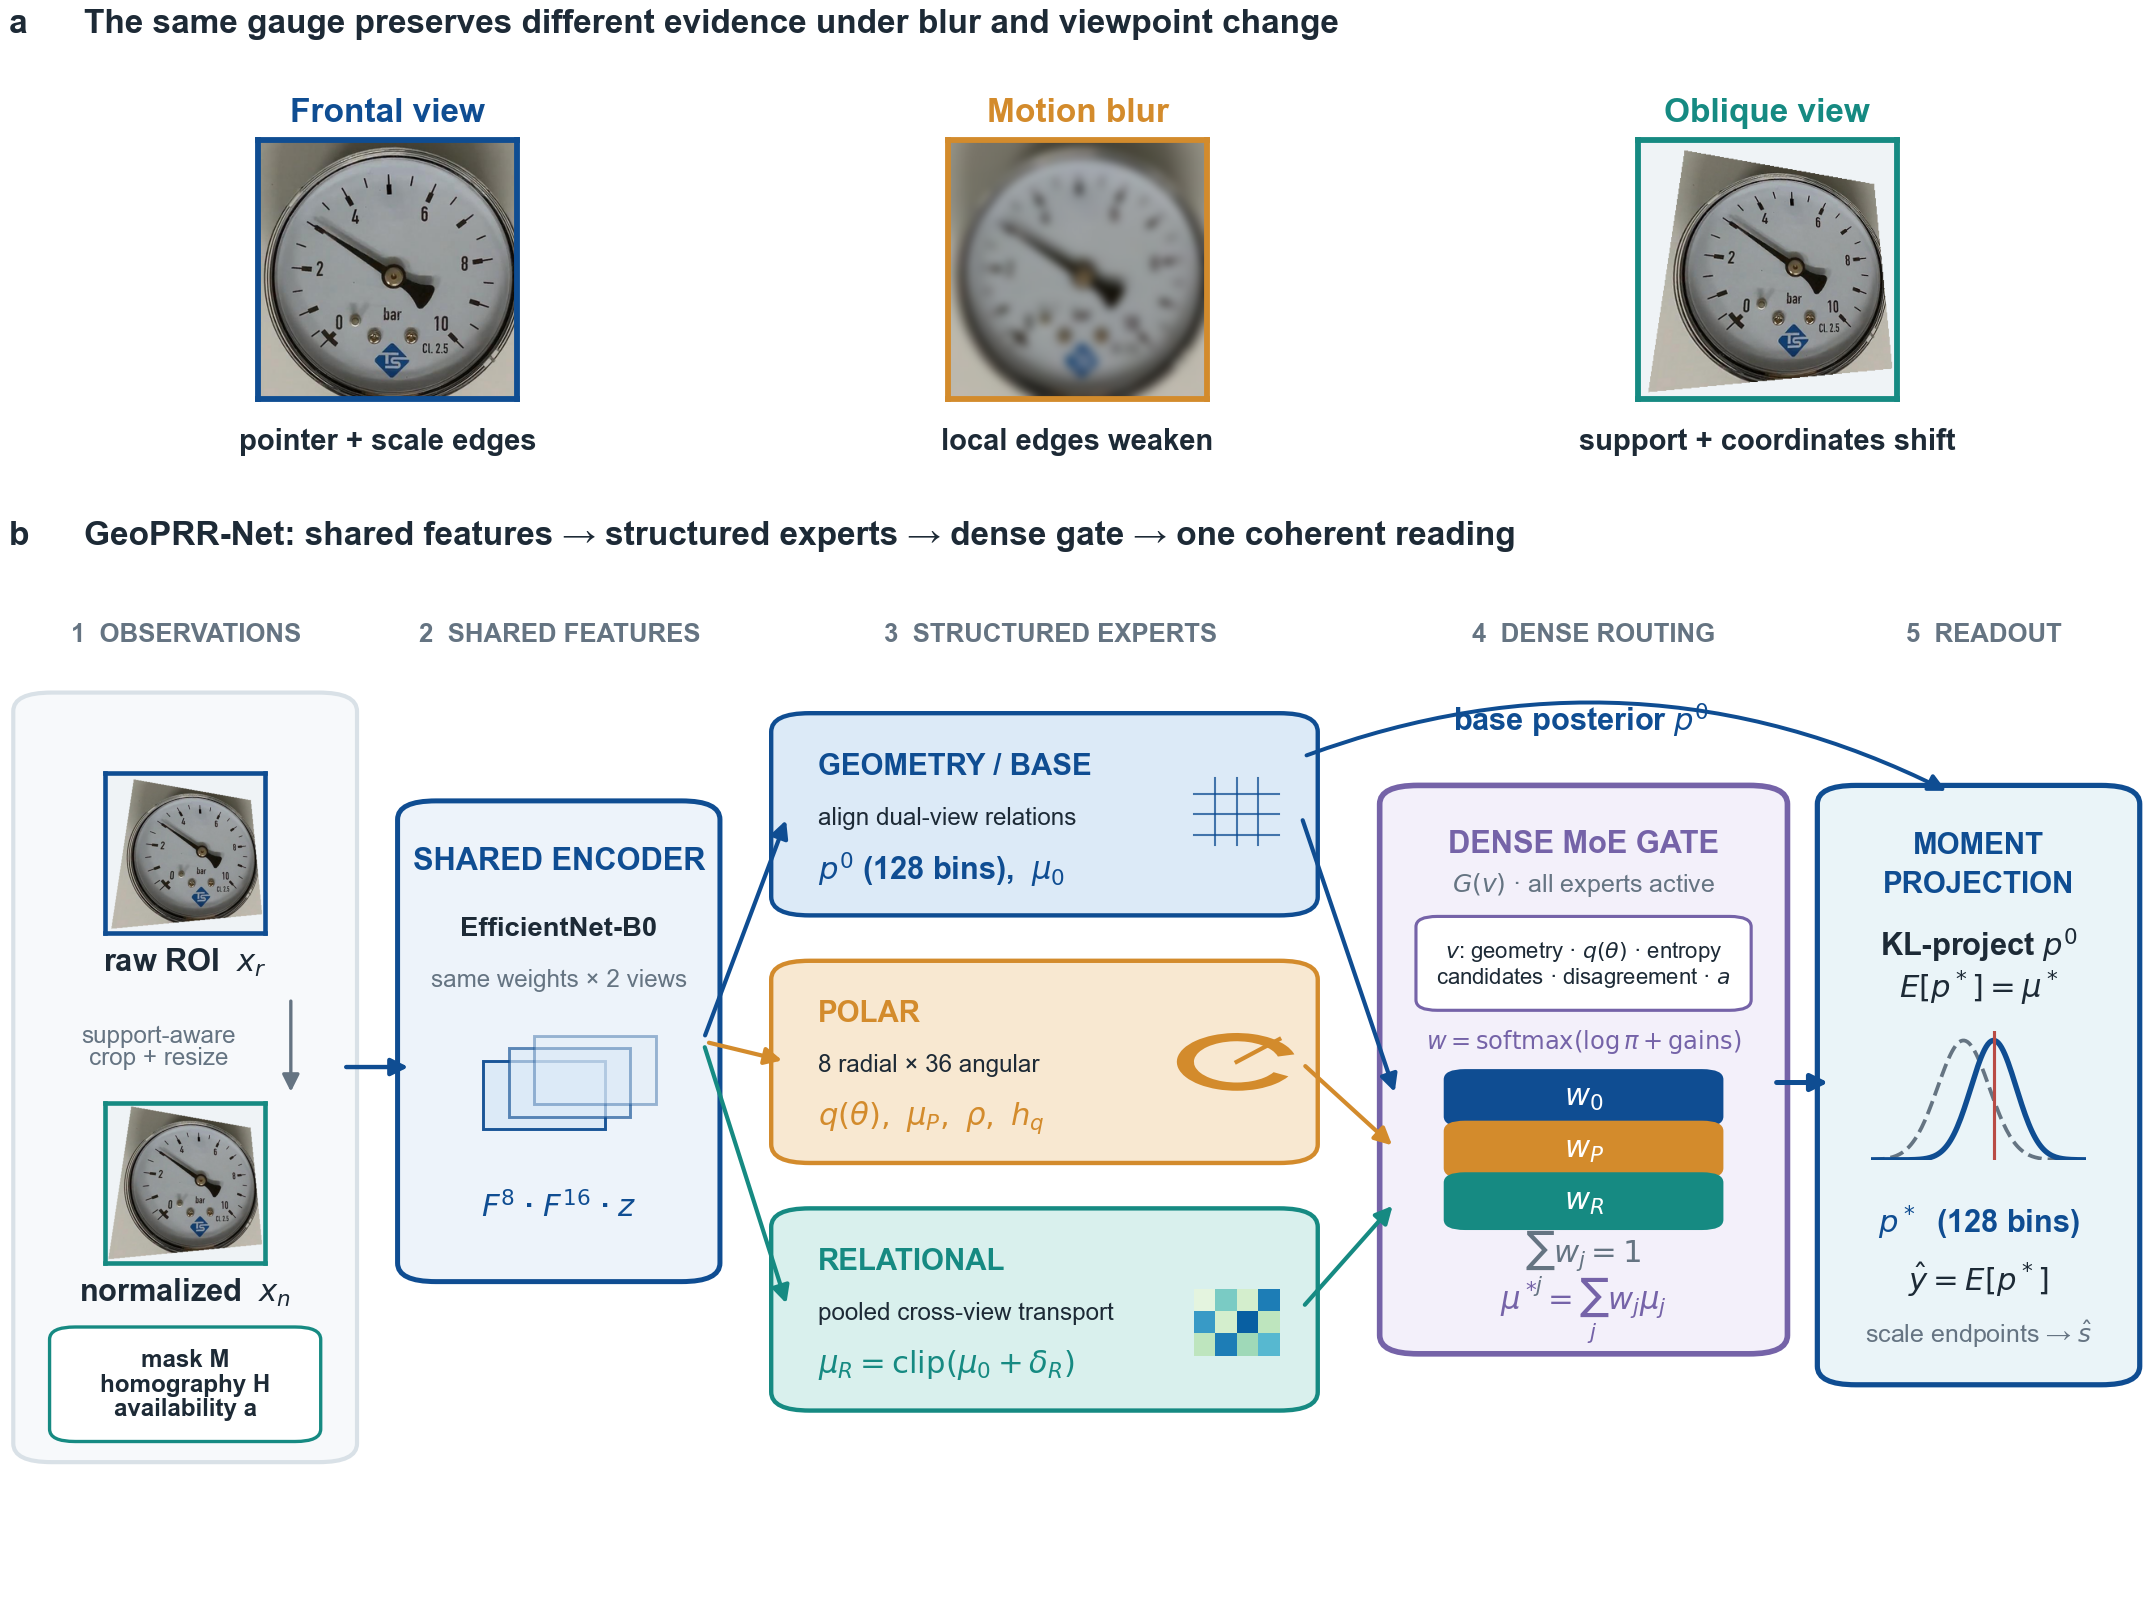
\includegraphics[width=\textwidth]{fig1_geoprr_architecture.png}
\caption{Field-capture challenge and dense-MoE evidence flow in \modelname. (\textbf{a}) One public RF100-VL gauge ROI \cite{robicheaux2025rf100vl} illustrates how frontal capture, motion blur, and an oblique viewpoint preserve different visual cues. (\textbf{b}) Support-aware normalization produces a second observation together with its mask, homography, and availability flag. A shared EfficientNet-B0 then supports geometry/base, polar, and relational experts with explicit candidate outputs. The dense input-dependent gate weights all three candidate means, while a KL information projection imposes the routed mean on the base posterior to return one coherent 128-bin posterior and final reading.}
\label{fig:architecture}
\end{figure}

\subsection{Shared Encoder and Geometry-Aware Base Expert}
\label{subsec:geometry}

EfficientNet-B0 was chosen as a compact, ImageNet-initialized foundation with multiscale spatial features and a global context representation \cite{tan2019efficientnet}. This hierarchy supports aligned dual-view geometry, polar sampling, and relational transport within one shared encoder. One parameter set processes $x_r$ and $x_n$ in two forward passes. We retain a stride-8 map with 40 channels, a stride-16 map with 112 channels, and a 1280-dimensional pooled context vector:
\begin{equation}
(F_r^8,F_r^{16},z_r)=E(x_r),\qquad (F_n^8,F_n^{16},z_n)=E(x_n).
\label{eq:encoder}
\end{equation}
The shared construction permits comparison between observations without doubling the backbone parameter count.

At each retained scale $l\in\{8,16\}$, $F_n^l$ is mapped into raw-view coordinates using $H_{r\rightarrow n}^{-1}$. Denote the aligned feature by $\widetilde{F}_n^l$ and the downsampled common-support mask by $M^l$. After channel projection, the relation tensor is
\begin{equation}
R^l=\left[F_r^l,\widetilde{F}_n^l,\widetilde{F}_n^l-F_r^l,
|\widetilde{F}_n^l-F_r^l|,F_r^l\odot\widetilde{F}_n^l,M^l\right].
\label{eq:relation}
\end{equation}
Signed difference retains direction, absolute difference represents discrepancy magnitude, and the product records agreement. Homography coefficients, valid-support fractions, availability, and preliminary scalar discrepancies form an additional geometry token. The masked multiscale memory conditions 128 progress-bin queries in a two-layer, four-head relation decoder. The decoder has a bounded moment budget of 0.025, preventing the geometry path from making an unbounded correction.

Let $t_k=k/(K-1)$ for $K=128$. The geometry/base expert returns a base distribution $p^0\in\Delta^{K-1}$ and candidate mean
\begin{equation}
\mu_0=\sum_{k=0}^{K-1}p_k^0t_k.
\label{eq:base_mean}
\end{equation}
Availability masking is applied before relation decoding. When Equation~\eqref{eq:fallback} is active, missing geometry cannot masquerade as a learned signal; the raw branch remains the reference state.

\subsection{Polar Evidence Expert}
\label{subsec:polar}

The polar path uses only raw-view feature maps, avoiding dependence on a successful support normalization. Stride-8 and stride-16 maps are projected to eight channels and sampled on a fixed grid containing eight radial and 36 angular bins. For each scale, zeroth and first radial moments are concatenated. Circular one-dimensional convolutions operate along angle and produce logits $q_j$ over angles $\theta_j=2\pi j/36$:
\begin{equation}
q_j=\frac{\exp(\ell_j)}{\sum_m\exp(\ell_m)},\qquad
d=\sum_j q_j[\sin\theta_j,\cos\theta_j].
\label{eq:polar_direction}
\end{equation}
The direction vector, concentration $\rho=\lVert d\rVert_2$, and entropy
\begin{equation}
h_q=-\frac{\sum_j q_j\log(q_j+10^{-7})}{\log 36}
\label{eq:polar_entropy}
\end{equation}
are concatenated with the flattened angular features and a projection of $z_r$. A compact fusion MLP predicts a logit residual relative to the raw scalar readout. The resulting sigmoid output is the polar expert's candidate mean $\mu_p\in[0,1]$. This expert makes angular regularity explicit, but it is not assumed to be reliable when the apparent center or support is poor.

\subsection{Relational Moment-Transport Expert}
\label{subsec:relational}

The relational expert summarizes cross-view context at a coarser level than the geometry decoder. A shared projection $\phi$ maps $z_r$ and $z_n$ to a latent representation. The input vector contains
\begin{equation}
u=\left[\phi(z_r),\phi(z_n),\phi(z_n)-\phi(z_r),
|\phi(z_n)-\phi(z_r)|,\phi(z_r)\odot\phi(z_n),g,s\right],
\label{eq:relational_features}
\end{equation}
where $g$ denotes geometry features and $s$ contains preliminary raw, normalized, and base readings and their differences. Layer-normalized GELU blocks predict bounded residual evidence. Internally, the expert retains mean-, tail-, and severe-condition summaries and combines them conservatively; the inference interface exposes one transported candidate mean
\begin{equation}
\mu_r=\operatorname{clip}(\mu_0+\delta_r,\epsilon,1-\epsilon),
\label{eq:relational_candidate}
\end{equation}
with $|\delta_r|\leq0.05$. This abstraction is intentional: the scientific intervention is the presence of relational moment transport, whereas separately naming every internal MLP would create nominal rather than causal ablations.

\subsection{Dense MoE Routing and Moment-Consistent Projection}
\label{subsec:routing}

Let $E_0$, $E_p$, and $E_r$ denote the geometry/base, polar, and relational experts, with candidate-mean vector $c=[\mu_0,\mu_p,\mu_r]$. Together they form a dense heterogeneous MoE: each expert operates on a distinct physical representation while reusing the shared image encoder. The conditional router is the MoE gating network. It receives the five latent cross-view relations in Equation~\eqref{eq:relational_features}, geometry features, the 36-bin polar posterior, concentration, entropy, candidate means, pairwise candidate differences, endpoint readings, and availability; denote this complete gate input by $v$. Its prior is
\begin{equation}
\pi=(0.50,0.25,0.25).
\label{eq:prior}
\end{equation}
A two-output gating network $G$ predicts bounded gains for polar and relational evidence. With $g_p,g_r=0.10\tanh(G(v))$, the three logits and weights are
\begin{equation}
L=\log\pi+\alpha[0,g_p,g_r],\qquad w=\operatorname{softmax}(L).
\label{eq:router}
\end{equation}
The routing scale $\alpha$ controls how strongly the predicted gains influence the expert weights and is set to 100 by default. Its sensitivity analysis is reported in Section~\ref{subsec:alpha_sensitivity}.
If an expert is removed in an ablation, its logit is masked and the remaining weights are renormalized exactly. The routed target is the convex mixture in normalized-progress moment space
\begin{equation}
\mu^*=\sum_{j\in\{0,p,r\}}w_j\mu_j.
\label{eq:routed_mean}
\end{equation}

Directly averaging expert posteriors would entangle evidence allocation with distributional shape. \modelname instead mixes only the candidate means, retains the geometry-aware base $p^0$, and solves the information projection
\begin{equation}
p^*=\arg\min_{p\in\Delta^{K-1}}D_{\mathrm{KL}}(p\Vert p^0)
\quad\text{subject to}\quad \sum_k p_kt_k=\mu^*.
\label{eq:iprojection}
\end{equation}
The solution has exponential-tilt form \cite{csiszar1975idivergence}:
\begin{equation}
p_k^*=\frac{p_k^0\exp(\lambda t_k)}{\sum_m p_m^0\exp(\lambda t_m)},
\label{eq:tilt}
\end{equation}
where Newton updates find $\lambda$ such that the first-moment constraint is satisfied to numerical tolerance. The final point prediction is $\widehat{y}=\sum_kp_k^*t_k$. The posterior is coherent with the routed scalar by construction; this consistency property is distinct from probabilistic calibration.

\subsection{Inference Graph and Parameter Inventory}
\label{subsec:inventory}

The inference sequence is deterministic once a checkpoint is loaded. First, the ROI is resized and the support-aware operation creates $(x_r,x_n,M,H_{r\rightarrow n},a)$. Second, the same encoder is called for both observations, and its intermediate features are retained. Third, aligned relation tokens produce $(p^0,\mu_0)$, the raw feature hierarchy produces $\mu_p$, and cross-view context produces $\mu_r$. Fourth, the gate computes $w$ from quantities available at inference; no label-dependent oracle signal is present. Fifth, Equation~\eqref{eq:routed_mean} yields one target mean. Finally, Equation~\eqref{eq:tilt} changes the base posterior only enough to satisfy that target. A failed support-normalization attempt sets $a=0$, activates the identity observation, and lets the raw, polar, and availability-aware paths continue.

Table~\ref{tab:parameters} records the unique learned parameter inventory. The shared dual-view geometry/base expert includes the only image encoder and accounts for 87.4\% of the checkpoint. The polar expert, relational expert, and conditional gate add 0.106, 0.442, and 0.065 million parameters, respectively. Thus, expert specialization is introduced primarily through lightweight evidence heads and a compact gate, while alignment, sampling, and moment projection account for the model's additional execution cost.

\begin{table}[H]
\caption{Unique parameter inventory for full \modelname. Shared tensors are counted once.}
\label{tab:parameters}
\centering
\small
\begin{tabularx}{0.78\textwidth}{@{}>{\raggedright\arraybackslash}Xrr@{}}
\toprule
\textbf{Component} & \textbf{Parameters} & \textbf{Share (\%)} \\
\midrule
Shared dual-view geometry/base expert & 4,271,638 & 87.44 \\
Polar evidence expert & 105,944 & 2.17 \\
Relational transport expert & 442,112 & 9.05 \\
Conditional gate & 65,402 & 1.34 \\
\midrule
Total & 4,885,096 & 100.00 \\
\bottomrule
\end{tabularx}
\end{table}

\subsection{Staged Expert and Router Fitting}
\label{subsec:training}

The complete network is fitted in ordered phases on the official 16,000-image SyncG training pool. Candidate modules and the final router each use all 16,000 images from 145 scenes, sharing the same source-training pool. Each source seed reuses its same-seed EfficientNet-B0 foundation trained on the full pool for 60 epochs. The warm-polar initializer was fitted once on the original 12,818-image subset using seed 20262020 and is shared across subsequent fits with seeds 20262020, 20262021, and 20262022. The polar phase uses ten epochs, batch size 64, AdamW learning rate $5\times10^{-4}$, weight decay $10^{-4}$, cosine annealing, mean absolute error, and a 0.10-weighted top-decile error term, with the other components frozen.

Expert outputs for all six conditions are then cached on the full source-training pool, producing 96,000 rows. Router stage one uses 40 epochs, batch size 512, AdamW at $10^{-3}$ with cosine annealing, and
\begin{equation}
\mathcal{L}_1=\mathcal{L}_{\mathrm{final\,L1}}+0.50\mathcal{L}_{\mathrm{gain}}
+0.25\mathcal{L}_{\mathrm{no\mbox{-}harm}}+0.002\mathcal{L}_{\mathrm{route}}.
\label{eq:router_stage1}
\end{equation}
The no-harm term penalizes degradation relative to the base on clean and blur-only conditions. Stage two runs 120 full-cache epochs at learning rate $3\times10^{-4}$ and optimizes mean condition error, a smooth worst-excess term, regression relative to the stage-one condition profile, polar consistency when the relation is unavailable, gain prediction, and a small route-classification term:
\begin{equation}
\mathcal{L}_2=\overline{e}_{c}+2\mathcal{L}_{\mathrm{worst}}+2\mathcal{L}_{\mathrm{reg}}
+0.20\mathcal{L}_{\mathrm{polar}}+0.25\mathcal{L}_{\mathrm{gain}}+0.001\mathcal{L}_{\mathrm{route}}.
\label{eq:router_stage2}
\end{equation}
Gradient norms are clipped at 5.0, and exponential parameter averaging with decay 0.995 is maintained within the recorded training trajectories. Source checkpoint selection uses fixed terminal budgets or predefined trajectory averages. The default routing scale remains 100 with prior $(0.50,0.25,0.25)$. Source checkpoints remain frozen throughout the SyncG and zero-shot comparisons. The retained Industrial adaptation protocol freezes the original source encoders and fits the same $128$--$64$ hidden-layer feature head for \modelname and the three raw CNNs, using dropout 0.1, a maximum of 100 epochs, and patience 20. Group-wise five-fold OOF predictions use validation Acc@5\%, then Acc@2\%, then negative NMAE for lexicographic selection, with earlier epochs winning ties. Single-seed OOF results and equal-weight three-seed prediction ensembles are reported separately.

\section{Experimental Protocol}
\label{sec:protocol}

\subsection{Datasets, Separation, and Perturbations}
\label{subsec:data}

SyncG is a synthetic analog-gauge benchmark with scene and structural annotations \cite{deng2026syncg}. We use all 16,000 official training images and the 4,000-image official test split. Training and test image identities are disjoint, while their 145 scene identities overlap. Each test image is evaluated under six deterministic conditions, yielding 24,000 image--condition rows per seed. The shared candidate/router training pool is described in Section~\ref{subsec:training}.

Industrial-1395 is a multi-collection field benchmark assembled from three working-scene photo collections. After provenance consolidation, it contains 1,395 labeled real-instrument ROIs organized into 52 acquisition groups. The same six-condition generator yields 8,370 rows. Its uncontrolled instrument appearance, viewpoint, illumination, and capture variation make the complete cohort the study's most application-proximal field evaluation. Two settings use this complete roster: frozen transfer without target-domain fitting and supervised group-wise five-fold OOF feature-head adaptation. Acquisition groups define the OOF partitions and preserve source dependence during bootstrap resampling.

For a public external transfer check, we use the 151-image test split of the \emph{needle-base-tip-min-max} gauge subset in RF100-VL \cite{robicheaux2025rf100vl}. Before model inference, box centers for the dial center, pointer tip, and minimum/maximum references are converted into directed angular progress. Of the 151 targets, 145 lie inside the annotated arc and six fall within a fixed $5^{\circ}$ endpoint tolerance and are clamped to the minimum; none is selected or rejected using model output. Conservative filename/source identity rules form 35 groups to avoid treating nearby video frames as independent. The same six conditions produce 906 rows per seed.

The six conditions are clean, moderate blur, severe blur, moderate perspective, severe perspective, and combined severe perspective plus blur. Blur uses Gaussian standard deviations of 0.0015 and 0.0030 times the image short side. Perspective uses a virtual-plane tilt of $25^{\circ}$ and $45^{\circ}$; the combined condition uses $45^{\circ}$ with severe blur. Axis and sign are fixed by sample identity, so all compared methods and seeds receive identical pixels.

Table~\ref{tab:cohorts} summarizes the evidence roles: an official source-domain test on SyncG, public-source transfer on RF100-VL, and complete-cohort field evaluation on Industrial-1395.

\begin{table}[H]
\caption{Datasets and evidence roles. Image counts are unique ROIs before the six-condition expansion. Industrial-1395 supplies field-acquired external evidence; RF100-VL supplies an independently sourced public transfer check.}
\label{tab:cohorts}
\centering
\small
\begin{tabularx}{\textwidth}{@{}>{\raggedright\arraybackslash}p{0.22\textwidth}>{\raggedright\arraybackslash}p{0.18\textwidth}>{\raggedright\arraybackslash}p{0.18\textwidth}>{\raggedright\arraybackslash}X@{}}
\toprule
\textbf{Cohort} & \textbf{Images / scenes} & \textbf{Rows per seed} & \textbf{Role and access rule} \\
\midrule
SyncG fitting population & 16,000 / 145 & Training-dependent & Candidate fitting and final-router fitting each use the full 16,000-image pool \\
SyncG official test & 4,000 / 145 & 24,000 & Source-domain evaluation; image identities are disjoint but scenes overlap with training \\
Industrial-1395 & 1,395 / 52 acquisition groups & 8,370 & Complete field cohort; frozen transfer and supervised group-wise five-fold OOF adaptation \\
RF100-VL gauge transfer & 151 / 35 source groups & 906 & Public six-condition transfer check; geometric target derived before inference; no adaptation \\
\bottomrule
\end{tabularx}
\end{table}

\subsection{External Baselines and Structured Comparators}
\label{subsec:baselines}

The seven readers are organized into two baseline families and the proposed method. The raw-regression family contains ResNet-18, EfficientNet-B0, and MobileNetV3-Large \cite{he2016resnet,tan2019efficientnet,howard2019mobilenetv3}. Each torchvision backbone ends in a sigmoid progress output. ResNet-18 and EfficientNet-B0 use ImageNet-1K V1 initialization, and MobileNetV3-Large uses ImageNet-1K V2. All three are fitted on the full 16,000-image source pool with $256\times256$ inputs, batch size 64, Smooth-L1 loss with $\beta=0.05$, AdamW, and weight decay $10^{-4}$. The 60-epoch schedule comprises 30 initial epochs at learning rate $3\times10^{-4}$ followed by 30 continuation epochs with the learning rate restarted at $3\times10^{-5}$; cosine decay is applied within the recorded phases.

The structured-reading family contains YOLO11s-Pose-4KP, DeepLabV3+-ROI, and VDN \cite{jocher2023ultralytics,chen2018deeplabv3plus,dong2021vdn}. YOLO predicts the pivot, pointer tip, and ordered scale endpoints. DeepLab predicts a pointer mask, and VDN predicts its direction. In all main comparisons, DeepLab and VDN obtain the pivot and scale endpoints from the same-seed source-trained YOLO model; its pointer-tip prediction is excluded from reference selection and conversion. Each structured method therefore produces a normalized reading from the supplied ROI without annotation-derived reference coordinates. Annotation-assisted DeepLab and VDN results are retained separately as component diagnostics in Appendix~\ref{app:annotation}.

Source budgets are fixed at 40 epochs for YOLO (30 initial plus 10 continuation), 20 for DeepLab, and 200 for VDN. YOLO and VDN use $384\times384$ network inputs and DeepLab uses $256\times256$. Checkpoints use the recorded terminal budget or predefined trajectory averaging rather than target-domain selection. VDN is retrained from ImageNet initialization on SyncG; it is not evaluated using an official pretrained gauge model. The three source seeds match those of \modelname.

Within each dataset, all seven methods use the same image--condition roster, normalized targets, and full scoring denominator. The comparison supplies the same ROI while allowing each reader its native internal computation. Sections~\ref{subsec:comparisons} and~\ref{subsec:zero_shot_results} first evaluate the official SyncG test split and then frozen transfer to the two real-image domains. Target-supervised OOF adaptation is evaluated separately with matched feature-head fitting and ensemble sizes.

\subsection{Expert-Mixture and Structural Ablations}
\label{subsec:ablation_protocol}

The retained interventions evaluate geometry-aware fusion, relational moment transport, and conditional routing (Table~\ref{tab:ablation_definitions}). Their original source candidate bank is shared across variants, with 12,818 images used for candidate fitting and 3,182 for final-router fitting. The geometry and relational interventions use the recorded 40-epoch and 120-epoch router-fitting stages on that router-training subset; the fixed-mixture control replaces the original full model's weights at inference. Removing an expert masks its logit and renormalizes the remaining simplex in Equation~\eqref{eq:router}. The fixed-mixture intervention retains the candidate predictions and replaces their input-dependent weights with $(0.50,0.25,0.25)$. The reported contrasts retain these variant measurements and use the updated full-source model from Section~\ref{subsec:training} as the full reference.

\begin{table}[H]
\caption{Compressed ablation definitions. The retained variants use their original fitting protocol; the reported full reference uses the updated full-source protocol. Data rosters, seeds, and evaluation pixels remain matched.}
\label{tab:ablation_definitions}
\centering
\small
\begin{tabularx}{\textwidth}{@{}>{\raggedright\arraybackslash}p{0.23\textwidth}>{\raggedright\arraybackslash}p{0.27\textwidth}X@{}}
\toprule
\textbf{Variant} & \textbf{Executable change} & \textbf{Question isolated} \\
\midrule
Full \modelname & All experts and input-dependent gating active & Complete proposed dense MoE \\
Without geometry-aware fusion & Replace the learned geometry base by an availability-aware mean of raw and normalized endpoint estimates; retain the relational displacement & Does learned aligned geometry, rather than merely creating a second view, matter? \\
Without relational transport & Remove the relational expert and renormalize over geometry/base and polar experts & Does cross-view moment transport add information beyond the base expert? \\
Fixed expert mixture & Keep all experts; use the fixed prior for every sample & Is an input-dependent gate better than a constant expert mixture? \\
\bottomrule
\end{tabularx}
\end{table}

\subsection{Metrics and Statistical Inference}
\label{subsec:statistics}

Because labels are normalized to full scale, the primary metric is
\begin{equation}
\nmae=\frac{1}{N}\sum_{i=1}^{N}|\widehat{y}_i-y_i|.
\label{eq:nmae}
\end{equation}
Equation~\eqref{eq:nmae} is computed on the normalized $[0,1]$ scale. Throughout the text, tables, and figures, we report $100\times\nmae$ as percent of full scale (\%FS); for example, an NMAE of 0.01 is reported as 1\%FS. Threshold accuracy is
\begin{equation}
\operatorname{Acc@}\tau=\frac{1}{N}\sum_i\mathbb{1}(|\widehat{y}_i-y_i|\leq\tau),
\label{eq:accuracy}
\end{equation}
with $\tau=0.01$, 0.02, and 0.05. The primary comparison tables report NMAE, Acc@5\%, and valid-reading coverage. Acc@5\% is the percentage of rows with absolute error at most 5\%FS. Failed readings retain normalized error 1.0, remain in the full denominator, and fail every accuracy threshold. Coverage measures whether a reading is returned, independently of whether it is accurate. Acc@1\%, Acc@2\%, RMSE, and error quantiles remain available in the released tables and prediction records.

Tables report the mean and sample standard deviation across the three source-seed fits unless a fixed ensemble is explicitly identified. These fits share the warm initializer described in Section~\ref{subsec:training}; a seed standard deviation is not a confidence interval. For paired comparisons, absolute errors are first averaged across seeds for each original image--condition row. Scene or acquisition/source groups are then resampled with replacement, retaining all constituent rows and their original weights \cite{davison1997bootstrap}. Percentile intervals use 20,000 replicates, with bootstrap seeds 20260907 for SyncG, 20261007 for RF100-VL, and 20261107 for Industrial. Relative reductions are recomputed within each replicate. We report $\Delta=100(\nmae_{\mathrm{GeoPRR}}-\nmae_{\mathrm{comparison}})$ in \%FS, so negative values favor \modelname. Ablation penalties reverse this order. Fixed three-member ensembles are scored after prediction averaging and compared with ensembles of the same size. Intervals are pointwise group-bootstrap intervals conditional on the fitted models.

Routing weights averaged across the three source-seed fits are used as mechanism diagnostics. Diagnostic expert preferences and prediction coverage are not measures of calibrated posterior uncertainty.

\subsection{Efficiency Measurement}
\label{subsec:efficiency_protocol}

Efficiency is measured on an NVIDIA GeForce RTX 4060 with CUDA 12.8 and PyTorch 2.11, using FP32 inference and batch size 1. Each complete reader receives 20 warm-up calls followed by 100 timed calls. The recorded boundary covers native preprocessing, transfers, executed networks, and conversion to a normalized reading. VDN and DeepLab include the source-trained reference detector. Model loading, file decoding, degradation synthesis, and accuracy scoring are outside this boundary. Accuracy uses the full six-condition rosters; the 100-call timing subset is a separate measurement.

We report loaded parameter counts, P50 and P95 latency, inverse-mean throughput, and peak allocated CUDA memory. All timed calls remain in the denominator. The frozen seven-reader comparison uses single source checkpoints; adapted single-model and equal-weight three-member ensemble timings are reported separately. THOP-supported operation counts are lower bounds because tensor-only transport, grid sampling, softmax, and other unsupported operations are omitted.

\section{Results}
\label{sec:results}

\subsection{Source-Domain Comparison on SyncG}
\label{subsec:comparisons}
\label{subsec:source}
\label{subsec:syncg_results}

Table~\ref{tab:syncg_external} and Figure~\ref{fig:syncg_overview} compare \modelname with three raw CNN regressors and three structured readers on the official SyncG test set. All seven methods use source-trained models and the complete six-condition ROI roster; VDN and DeepLab use automatic reference geometry. \modelname achieved the lowest pooled NMAE and highest Acc@5\%. Relative to EfficientNet-B0, the lowest-error raw CNN, its NMAE was reduced by 55.4\%, with a paired difference of $-0.9188$\%FS (95\% CI $[-0.9610,-0.8783]$\%FS). The corresponding reduction relative to VDN, the lowest-error structured reader, was 85.2\%. The agreement between lower continuous error and higher threshold accuracy indicates that the advantage extends to the fraction of readings meeting the specified tolerance. Coverage remained complete, so this performance was obtained over the full evaluation roster.

\begin{table}[H]
\caption{Source-only comparison on the official SyncG test set: 4,000 images, 145 scene groups, and 24,000 image--condition rows per seed. All references are automatic. Values are mean $\pm$ sample SD over three seeds. NMAE is in \%FS; Acc@5\% and valid-reading coverage are percentages. Failed readings retain normalized error 1.0 and remain in the denominator. Bold marks the lowest NMAE.}
\label{tab:syncg_external}
\centering
\small
\begin{tabularx}{\textwidth}{@{}>{\raggedright\arraybackslash}Xccc@{}}
\toprule
\textbf{Method} & \textbf{NMAE $\downarrow$} & \textbf{Acc@5\% $\uparrow$} & \textbf{Coverage $\uparrow$} \\
\midrule

\multicolumn{4}{@{}l}{\textit{Raw CNN regressors}} \\
Raw ResNet-18 & $2.4914\pm0.0564$ & $85.92\pm0.21$ & $100.00\pm0.00$ \\
Raw EfficientNet-B0 & $1.6595\pm0.0627$ & $93.96\pm0.59$ & $100.00\pm0.00$ \\
Raw MobileNetV3-Large & $2.3340\pm0.1864$ & $88.10\pm0.95$ & $100.00\pm0.00$ \\
\addlinespace\multicolumn{4}{@{}l}{\textit{Structured readers with automatic references}} \\
YOLO11s-Pose-4KP & $5.7478\pm2.1936$ & $82.24\pm2.22$ & $97.63\pm2.66$ \\
VDN & $5.0129\pm2.5266$ & $83.37\pm2.69$ & $97.63\pm2.66$ \\
DeepLabV3+-ROI & $10.2757\pm2.6382$ & $80.02\pm2.46$ & $94.96\pm2.69$ \\
\addlinespace
\modelname & $\mathbf{0.7407\pm0.0220}$ & $98.90\pm0.04$ & $100.00\pm0.00$ \\

\bottomrule
\end{tabularx}
\end{table}

Figure~\ref{fig:syncg} examines how the overall advantage behaves when the same images are perturbed. The matched clean-to-distorted comparisons in panel (\textbf{a}) show small mean changes under blur and larger changes under perspective distortion. Under combined severe distortion, the mean error increase was 0.4306\%FS for \modelname and 2.8099\%FS for EfficientNet-B0. Thus, the separation between these readers includes a lower cost of geometric perturbation, which directly addresses the oblique-viewpoint challenge of gauge reading. The comparison uses each image's own clean result as the reference, reducing the influence of differences in the underlying meter content.

Panels (\textbf{b},\textbf{c}) examine whether that lower error translates into more usable readings and persists beyond one threshold. At the 5\%FS tolerance, \modelname recovered 5.02\% of all image--condition rows relative to EfficientNet-B0 while losing 0.08\%. Corrections therefore substantially outnumbered newly incorrect readings. Across the displayed nonzero tolerance grid, its three-seed mean correct-reading fraction remained above all six comparators, indicating that the observed ranking was not confined to the selected 5\%FS operating point. Annotation-assisted VDN and DeepLab results remain separate in Appendix~\ref{app:annotation_diagnostic}.

\begin{figure}[H]
\centering
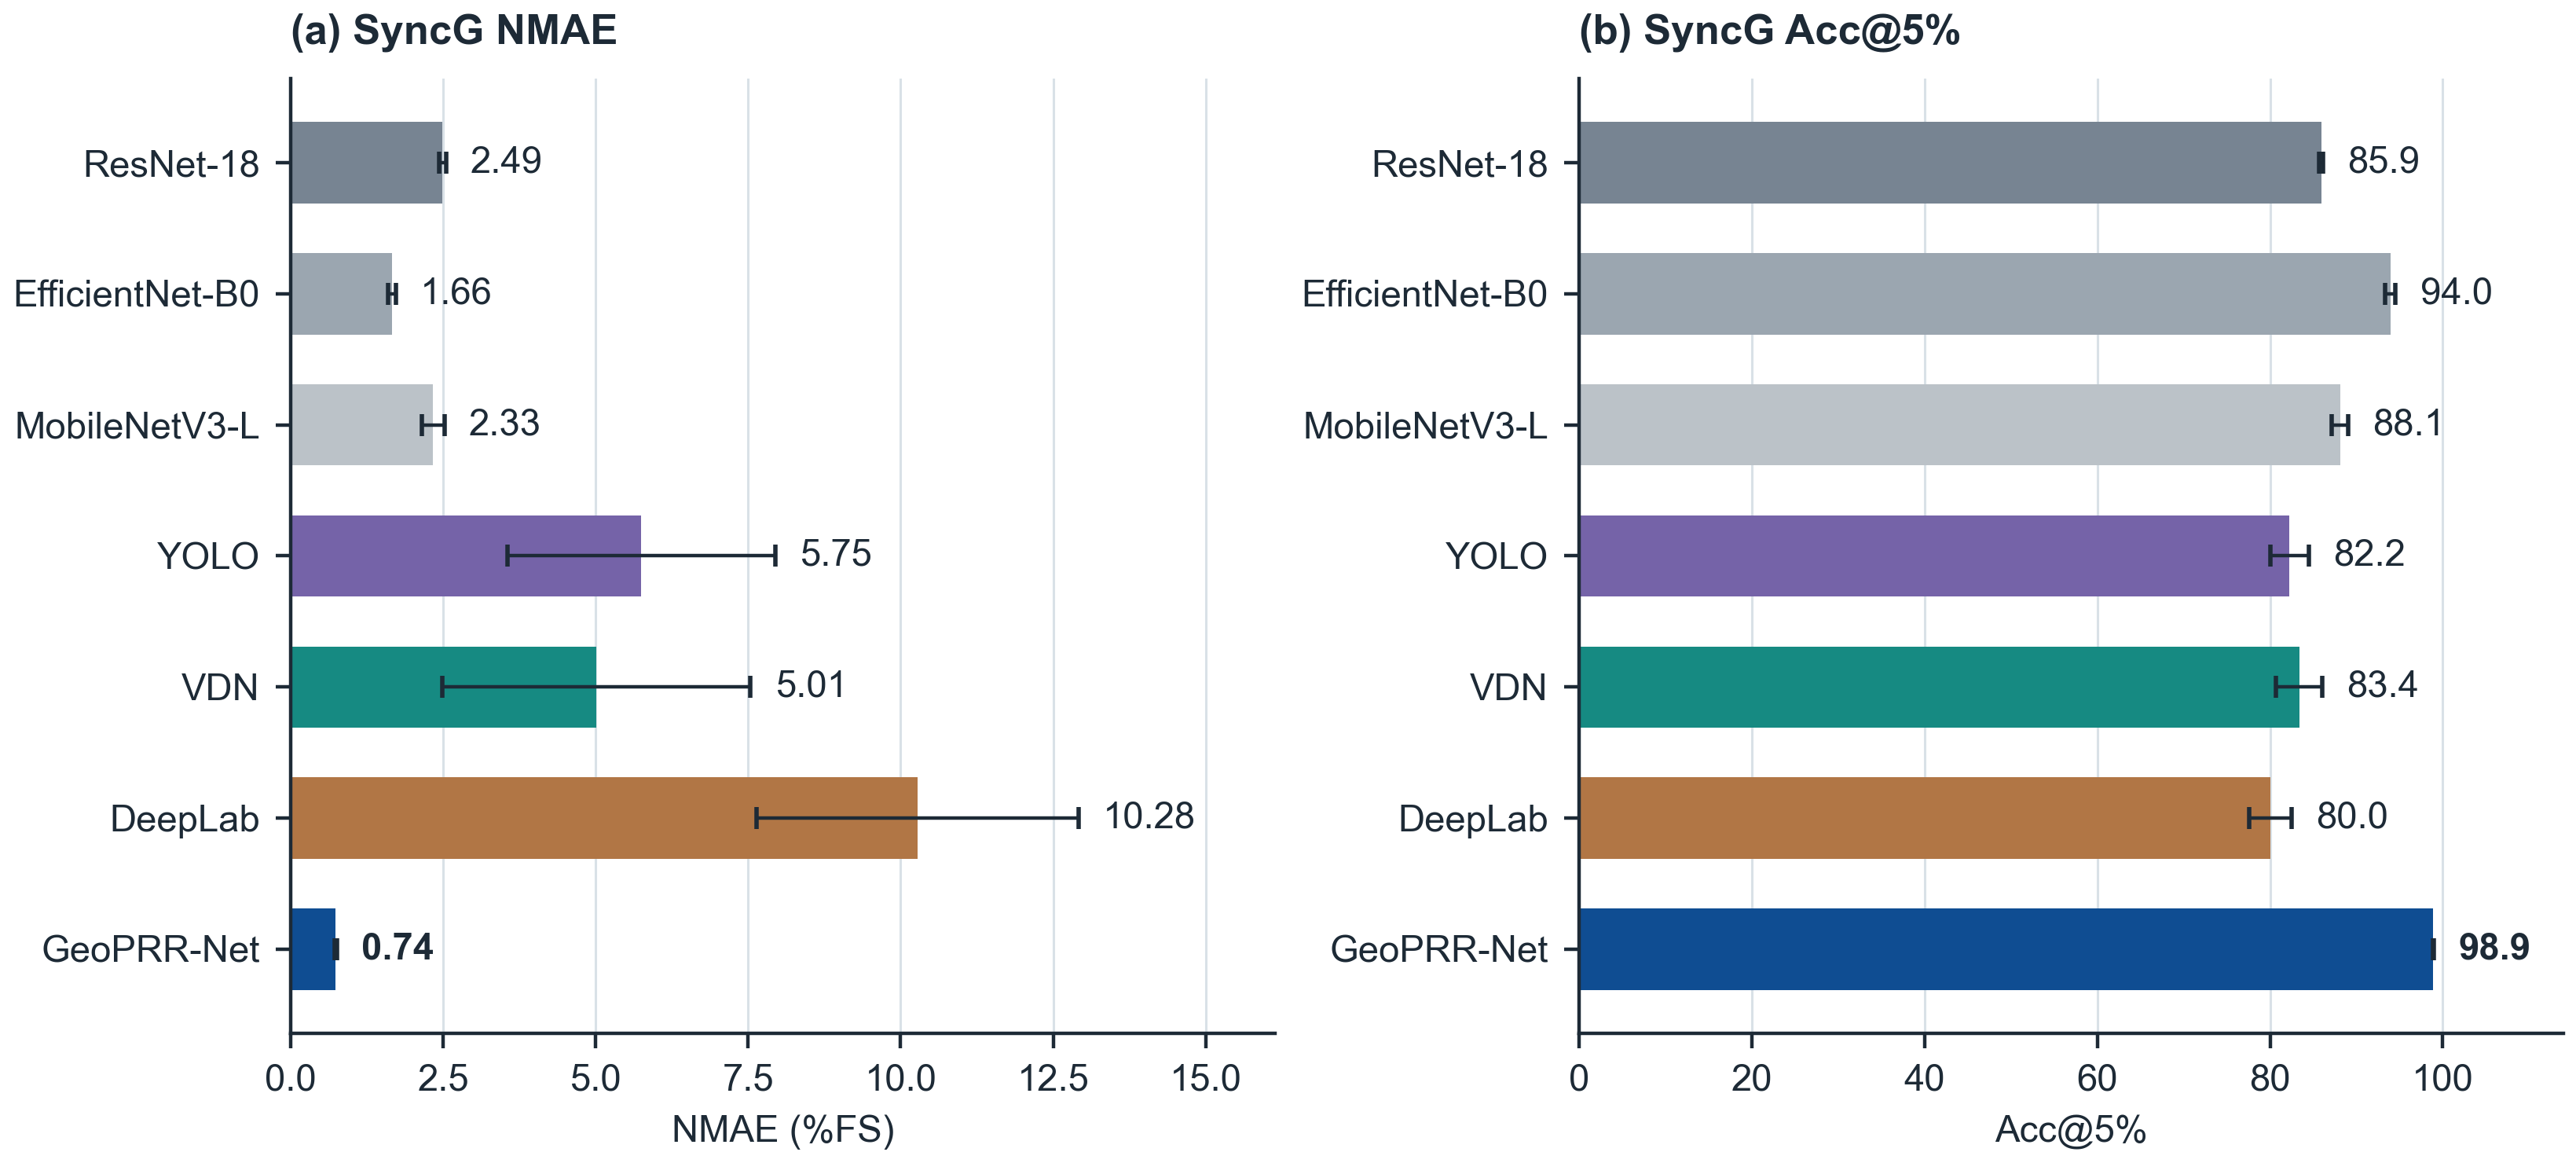
\includegraphics[width=\textwidth]{fig_syncg_overview.png}
\caption{Pooled SyncG comparison of seven source-trained readers. (\textbf{a}) NMAE in \%FS; lower is better. (\textbf{b}) Acc@5\% in percent; higher is better. Bars and whiskers show means and sample standard deviations over the three source seeds on the complete 24,000-row image--condition roster. Structured readers use automatic reference geometry.}
\label{fig:syncg_overview}
\end{figure}

\begin{figure}[H]
\centering
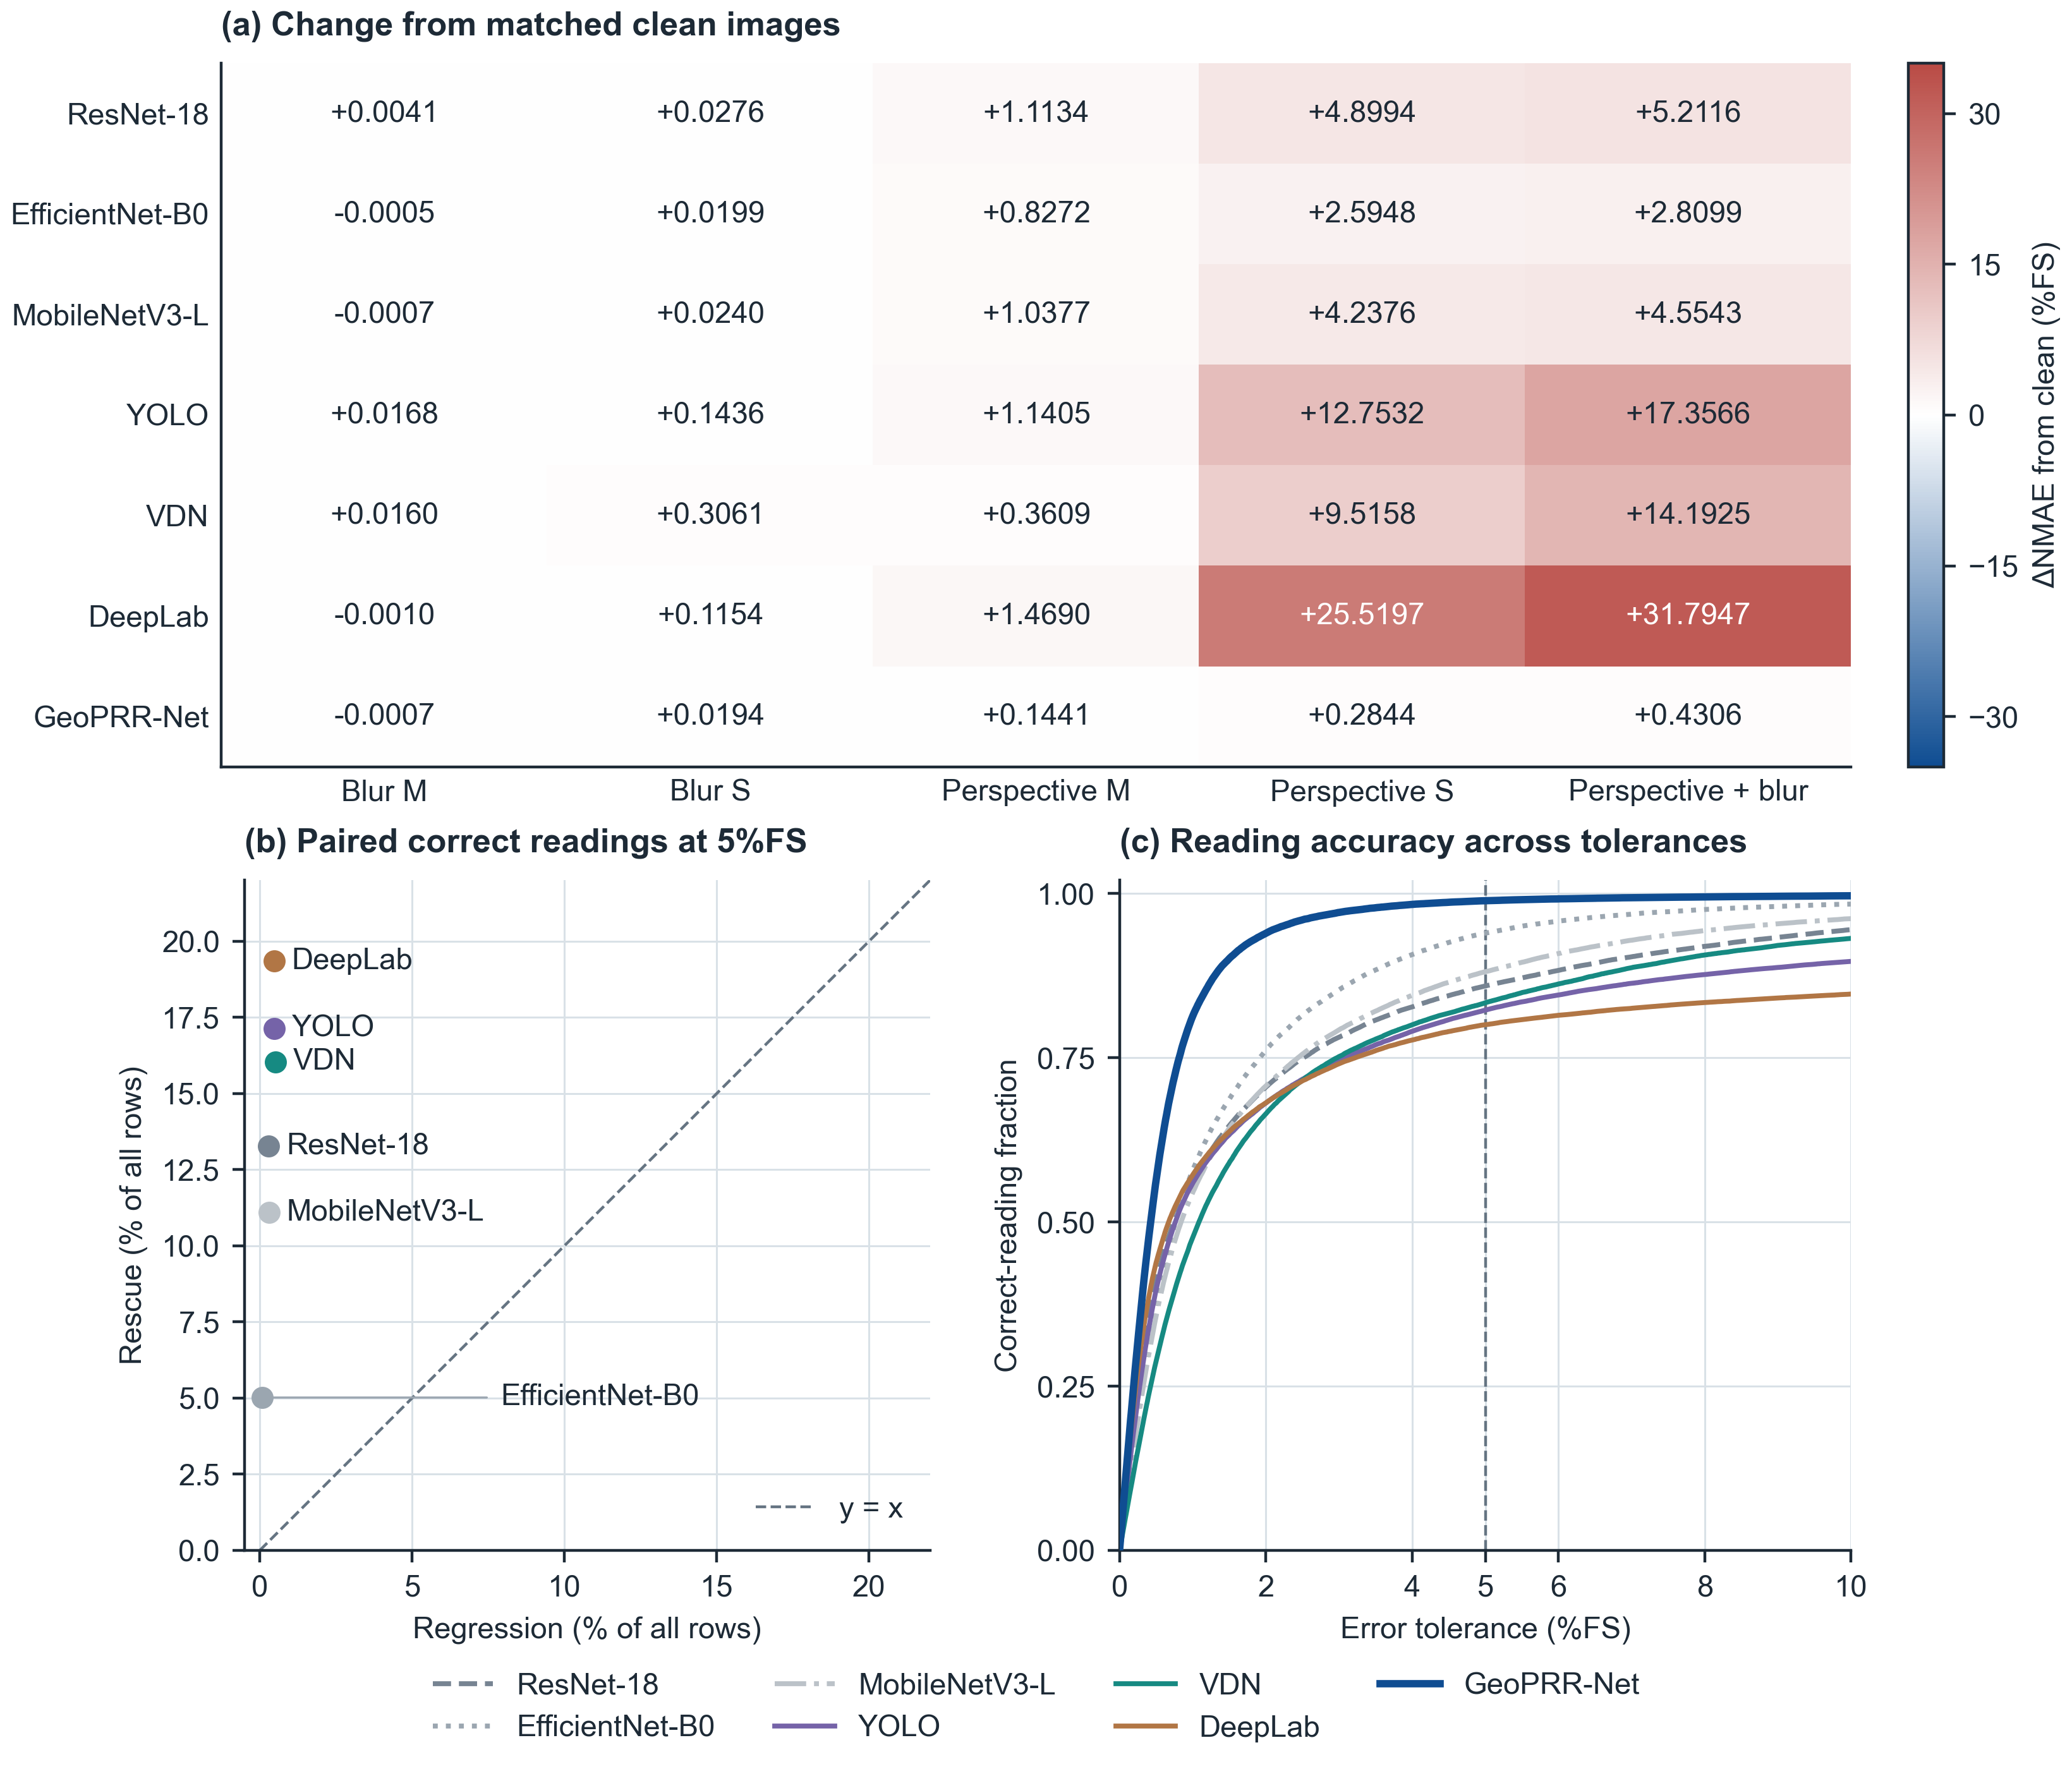
\includegraphics[width=\textwidth]{fig_syncg_evidence.png}
\caption{Paired robustness and reading accuracy on SyncG. (\textbf{a}) Mean change in absolute reading error from the same clean image for each perturbation, computed within each source seed and then averaged over 4,000 images and three seeds. Positive changes indicate increased error. (\textbf{b}) Paired outcomes at a 5\%FS tolerance: a rescue occurs when the comparator is incorrect and \modelname is correct; a regression reverses these outcomes. Points are means of the three seed-specific rates over all 24,000 rows per seed; the diagonal denotes equal rescue and regression. (\textbf{c}) Mean correct-reading fraction over three seeds as the tolerance varies from 0 to 10\%FS. Failed readings remain in the denominator and never count as correct. The curves at 5\%FS reproduce Acc@5\%. Panels (\textbf{b},\textbf{c}) show means without uncertainty bars or bands.}
\label{fig:syncg}
\end{figure}

\subsection{Zero-Shot Transfer to Real-Image Cohorts}
\label{subsec:transfer}
\label{subsec:zero_shot_results}

The same seven frozen source-trained readers are evaluated on RF100-VL and Industrial-1395 without target-domain training (Table~\ref{tab:zero_shot}). On Industrial-1395, \modelname has the lowest pooled NMAE, reducing error by 15.1\% relative to EfficientNet-B0; the paired difference is $-2.0679$\%FS (95\% CI $[-2.6474,-1.4428]$\%FS). It also has lower NMAE than each structured reader under automatic reference geometry.

\begin{table}[H]
\caption{Zero-shot transfer of all seven source-trained methods. RF100-VL contains 151 images from 35 source groups (906 rows per seed); Industrial-1395 contains 1,395 native ROIs from 52 acquisition groups (8,370 rows per seed). Both cohorts use all six conditions and automatic references. Values are three-seed mean $\pm$ sample SD; NMAE is in \%FS, and Acc@5\% and coverage are percentages. No target-domain adaptation is used. Bold marks the lowest NMAE within each cohort.}
\label{tab:zero_shot}
\centering
\small
\begin{tabularx}{\textwidth}{@{}>{\raggedright\arraybackslash}Xccc@{}}
\toprule
\textbf{Method} & \textbf{NMAE $\downarrow$} & \textbf{Acc@5\% $\uparrow$} & \textbf{Coverage $\uparrow$} \\
\midrule
\multicolumn{4}{@{}l}{\textbf{RF100-VL}} \\

\multicolumn{4}{@{}l}{\textit{Raw CNN regressors}} \\
Raw ResNet-18 & $7.8510\pm0.5142$ & $56.84\pm4.43$ & $100.00\pm0.00$ \\
Raw EfficientNet-B0 & $4.6057\pm0.5570$ & $74.36\pm2.74$ & $100.00\pm0.00$ \\
Raw MobileNetV3-Large & $5.9418\pm1.0743$ & $66.30\pm2.19$ & $100.00\pm0.00$ \\
\addlinespace\multicolumn{4}{@{}l}{\textit{Structured readers with automatic references}} \\
YOLO11s-Pose-4KP & $17.8599\pm5.1479$ & $52.06\pm1.63$ & $94.89\pm5.42$ \\
VDN & $19.6971\pm6.6315$ & $52.28\pm6.34$ & $94.89\pm5.42$ \\
DeepLabV3+-ROI & $30.4040\pm2.6979$ & $45.81\pm1.70$ & $85.54\pm2.65$ \\
\addlinespace
\modelname & $\mathbf{3.2053\pm0.2535}$ & $85.14\pm0.23$ & $100.00\pm0.00$ \\

\midrule
\multicolumn{4}{@{}l}{\textbf{Industrial-1395}} \\

\multicolumn{4}{@{}l}{\textit{Raw CNN regressors}} \\
Raw ResNet-18 & $22.0201\pm0.9947$ & $24.51\pm3.20$ & $100.00\pm0.00$ \\
Raw EfficientNet-B0 & $13.6914\pm2.4021$ & $41.40\pm4.17$ & $100.00\pm0.00$ \\
Raw MobileNetV3-Large & $16.4371\pm4.6792$ & $33.74\pm6.64$ & $100.00\pm0.00$ \\
\addlinespace\multicolumn{4}{@{}l}{\textit{Structured readers with automatic references}} \\
YOLO11s-Pose-4KP & $32.6975\pm6.4584$ & $36.13\pm1.80$ & $89.41\pm8.29$ \\
VDN & $33.0519\pm8.6304$ & $36.89\pm4.95$ & $89.41\pm8.29$ \\
DeepLabV3+-ROI & $39.4753\pm1.8138$ & $35.68\pm3.29$ & $76.40\pm0.97$ \\
\addlinespace
\modelname & $\mathbf{11.6235\pm1.6030}$ & $51.81\pm3.34$ & $100.00\pm0.00$ \\

\bottomrule
\end{tabularx}
\end{table}

On RF100-VL, \modelname achieved the lowest NMAE among all seven readers. The \modelname-minus-EfficientNet difference was $-1.4005$\%FS (95\% CI $[-1.8858,-1.0286]$\%FS); the difference from MobileNetV3-Large was $-2.7365$\%FS (95\% CI $[-3.5822,-2.0672]$\%FS). Both intervals were below zero. Figure~\ref{fig:zero_shot_overview} shows that the lower NMAE was accompanied by higher Acc@5\% in both target cohorts. The same source-trained reader therefore retained an advantage in both mean error and the proportion of tolerance-qualified readings after transfer to real images. These frozen-transfer results provide the reference for the target-domain readout comparison in Section~\ref{subsec:industrial_results}.

Figure~\ref{fig:zero_shot_visual} separates paired reading outcomes from the distribution of gains across source or acquisition groups. In panels (\textbf{a},\textbf{b}), mean recovery exceeded mean loss for every comparator in both cohorts. On Industrial-1395, the comparison with frozen EfficientNet-B0 recovered 12.95\% of all image--condition rows and lost 2.55\%, yielding a net Acc@5\% improvement of 10.41 percentage points. This establishes an improvement in tolerance-qualified readings on matched inputs, complementing the NMAE comparison with direct evidence that more readings meet the evaluation criterion.

Panels (\textbf{c},\textbf{d}) show the breadth of those gains. On RF100-VL, \modelname reduced group-mean NMAE in at least 32 of the 35 source groups against every comparator. On Industrial-1395, the advantage over each structured reader extended to all 52 acquisition groups, while 38 groups improved relative to EfficientNet-B0. All six image-weighted overall NMAE gains on this cohort had group-bootstrap intervals above zero. The agreement between the pooled results and their broad coverage across groups strengthens the evidence for transferable reading capability within the evaluated real-image cohorts.

\begin{figure}[H]
\centering
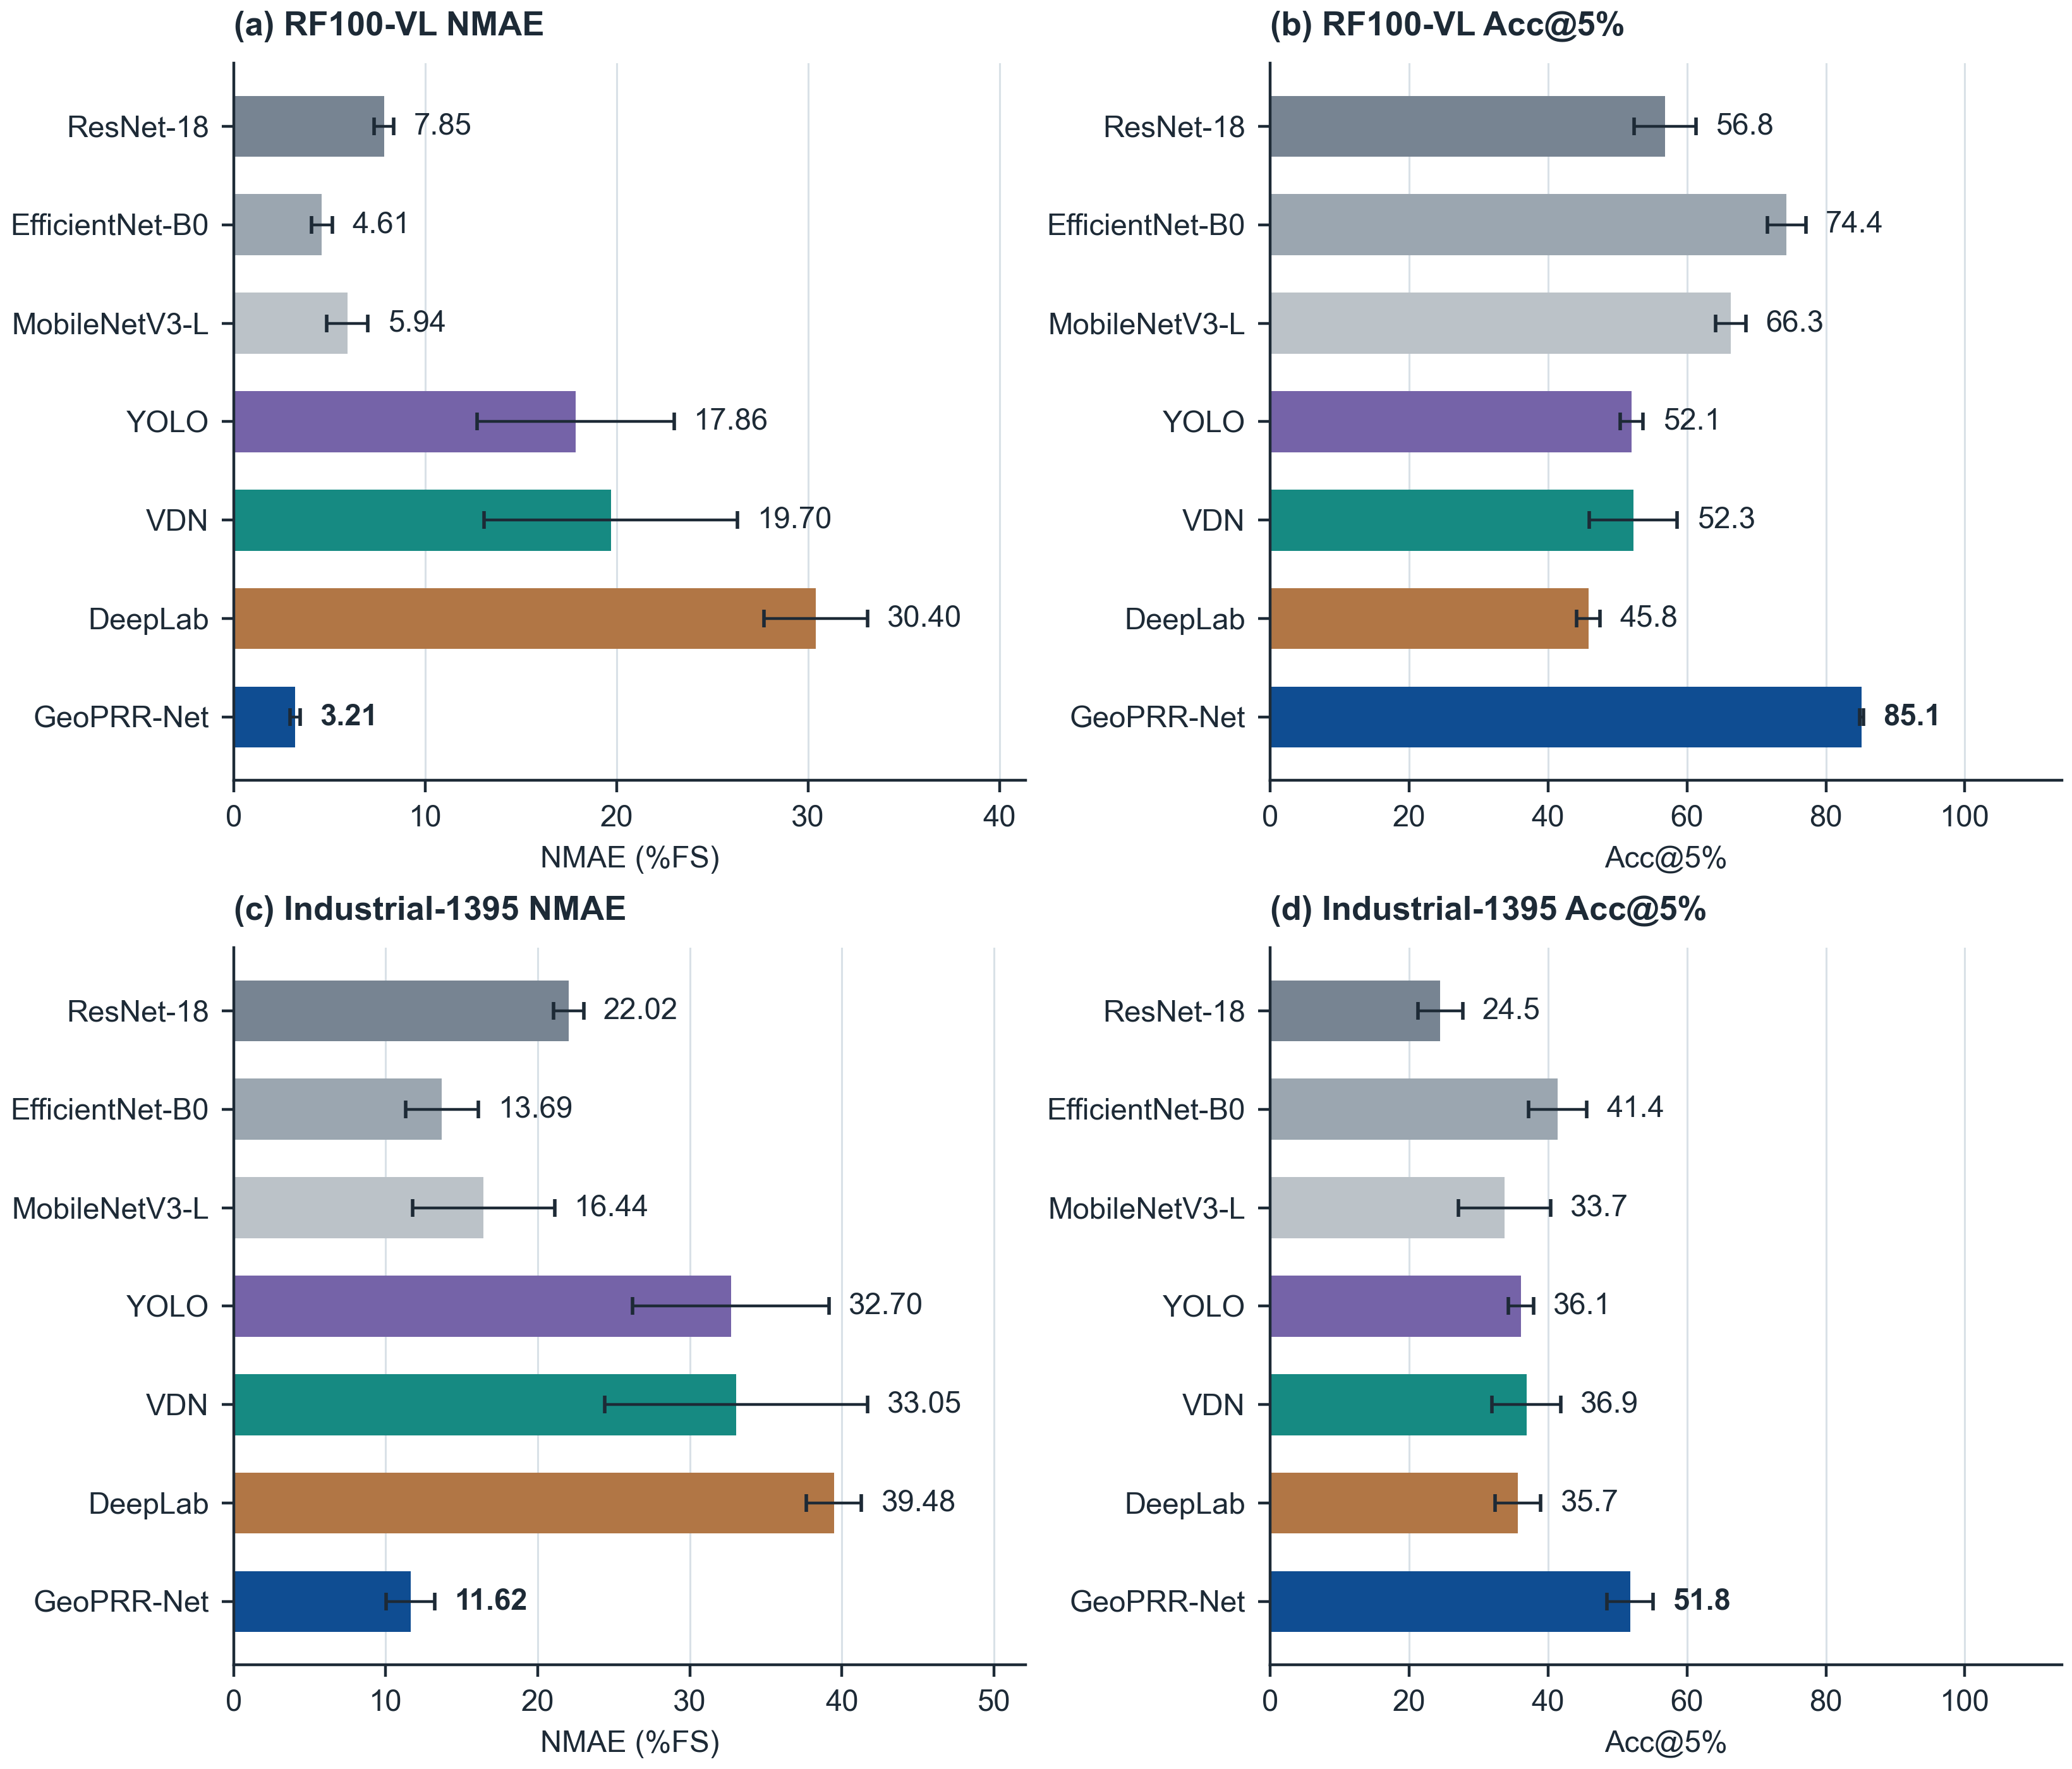
\includegraphics[width=\textwidth]{fig_zero_shot_overview.png}
\caption{Pooled zero-shot performance of seven frozen source-trained readers. (\textbf{a},\textbf{b}) RF100-VL NMAE and Acc@5\%. (\textbf{c},\textbf{d}) Industrial-1395 NMAE and Acc@5\%. Bars and whiskers are means and sample standard deviations over three seeds. Both domains use all six conditions, the full scoring denominator, and automatic reference geometry. NMAE is in \%FS and Acc@5\% is in percent.}
\label{fig:zero_shot_overview}
\end{figure}

\begin{figure}[H]
\centering
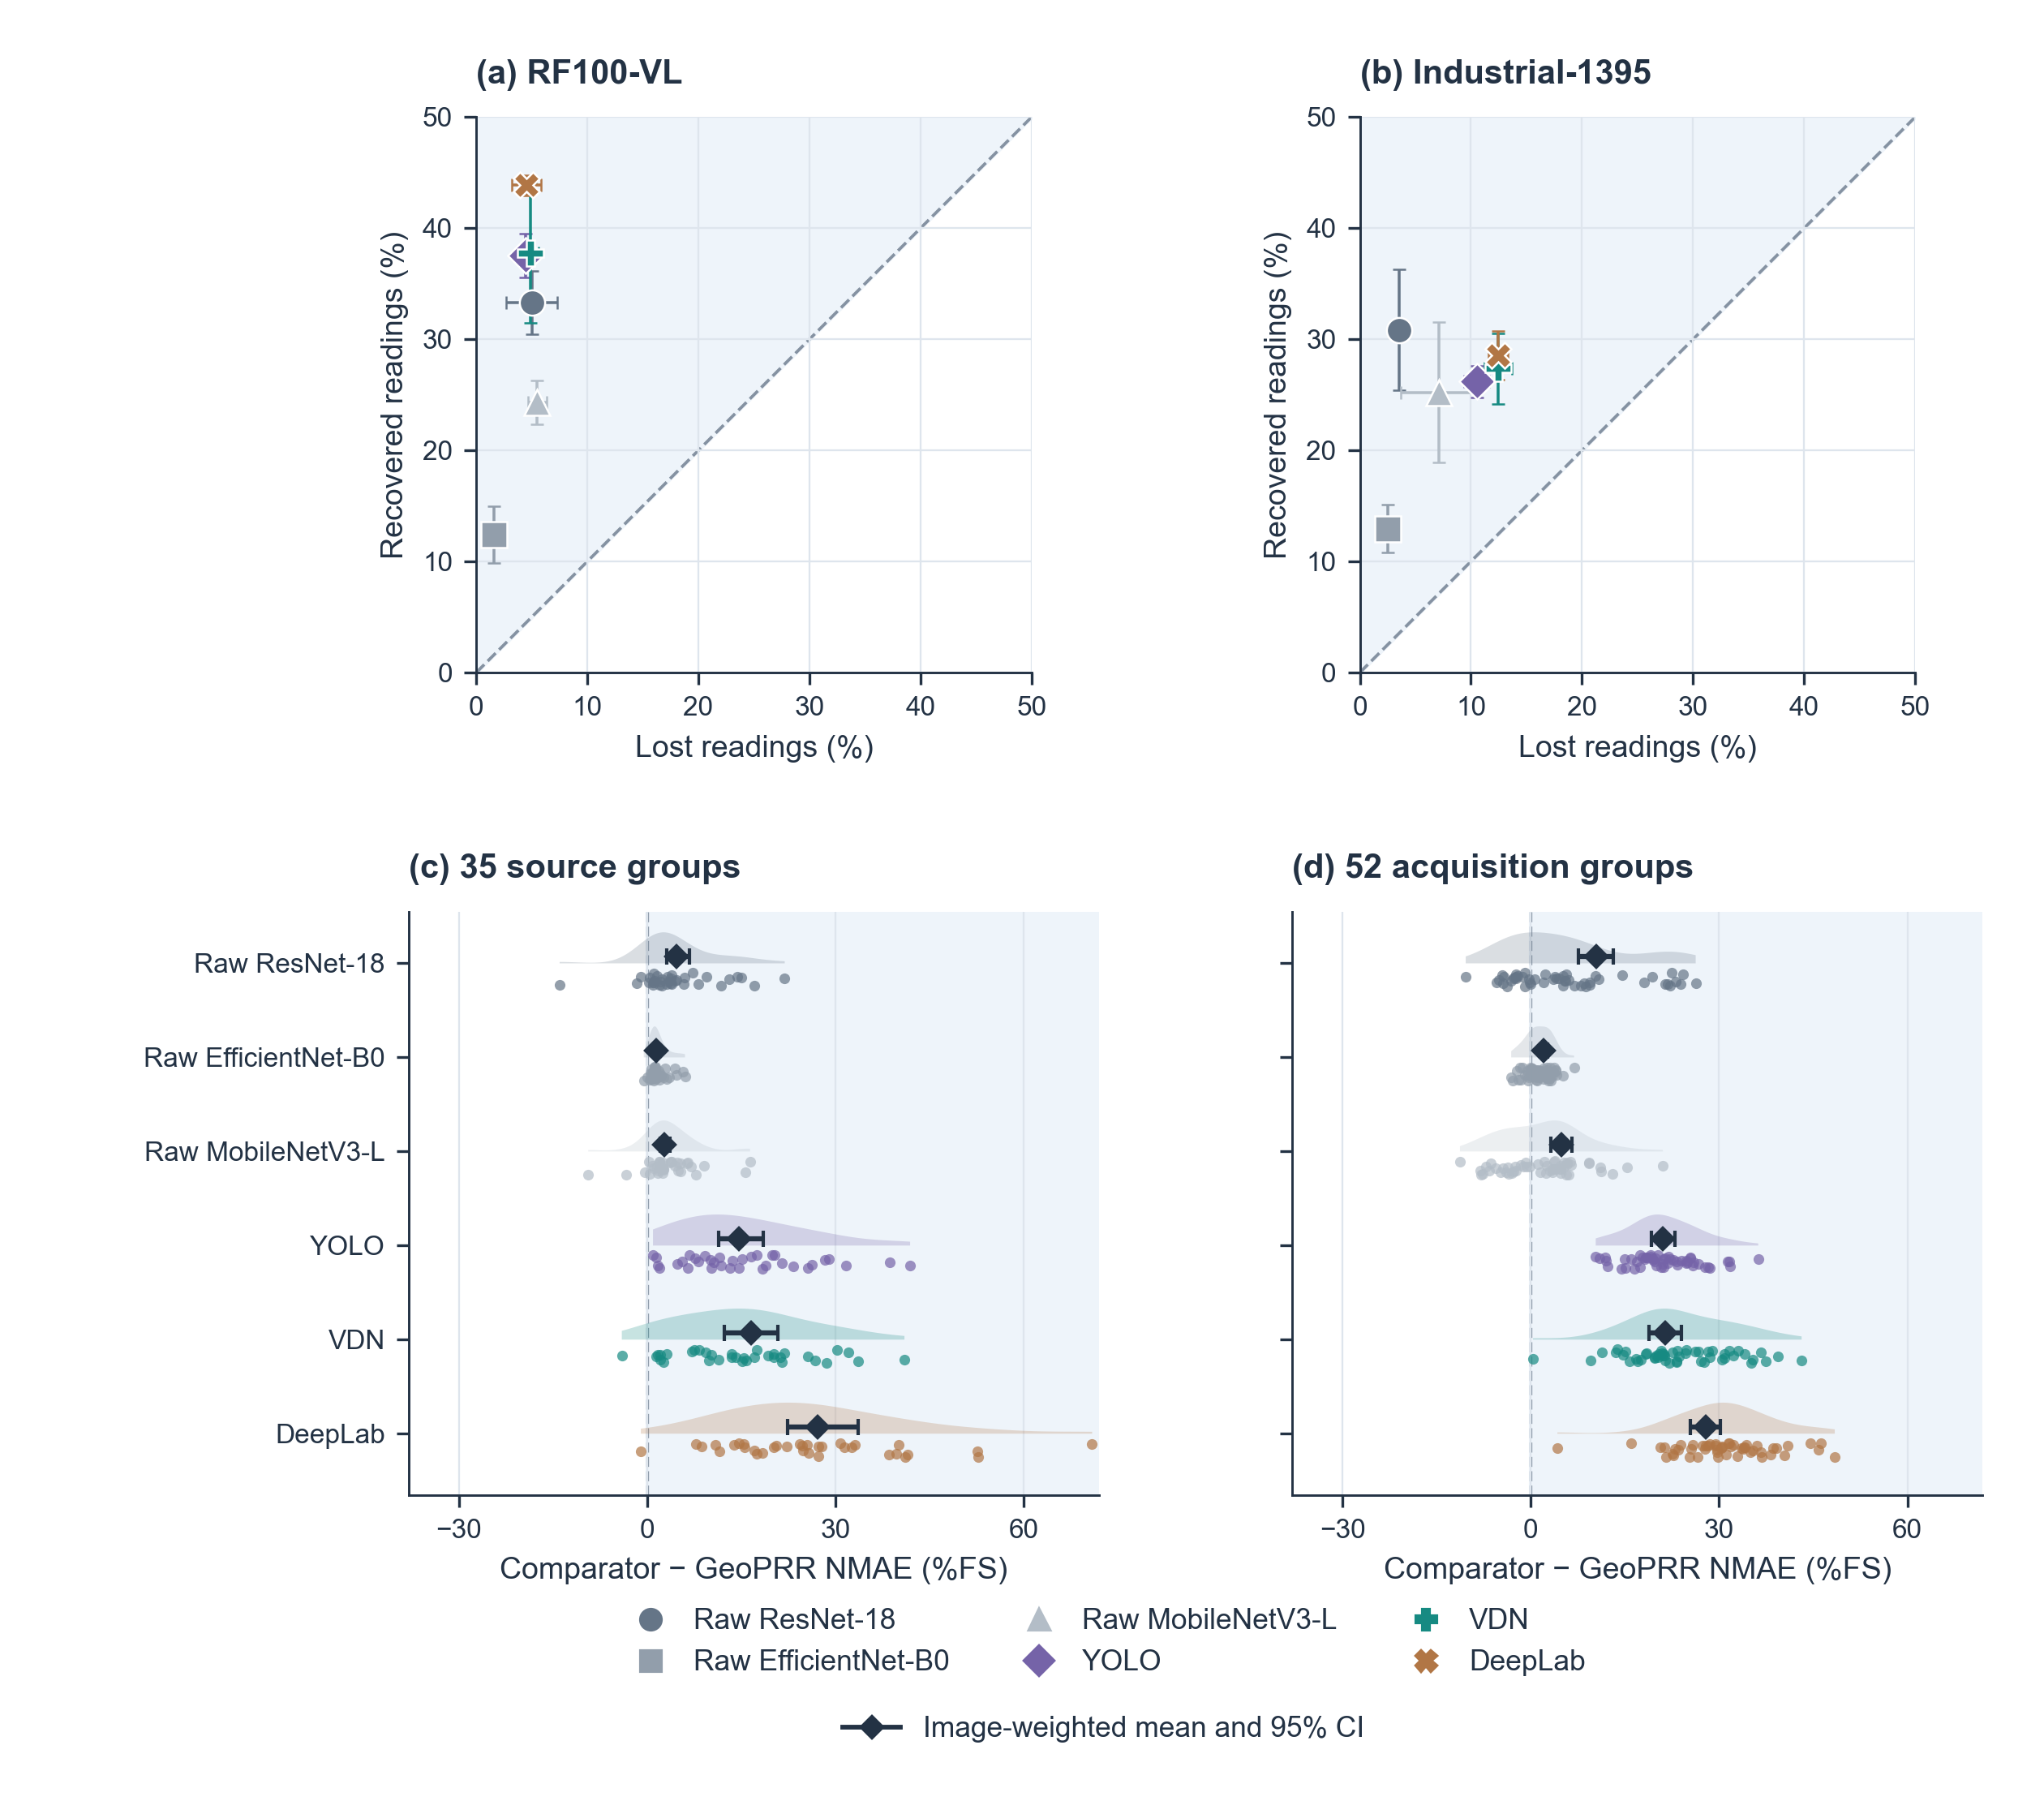
\includegraphics[width=\textwidth]{fig_zero_shot_evidence.png}
\caption{Paired reading outcomes and group-level zero-shot effects. (\textbf{a},\textbf{b}) RF100-VL and Industrial-1395 recovered-versus-lost reading rates at a 5\%FS tolerance. Recovery denotes a comparator-incorrect/\modelname-correct pair, and loss denotes the reverse; correctness requires a valid prediction within the tolerance. Points and horizontal and vertical whiskers are means and sample standard deviations of the three seed-specific rates. The diagonal denotes equal recovery and loss. (\textbf{c},\textbf{d}) Paired NMAE gains for all 35 RF100-VL source groups and 52 Industrial acquisition groups. Each dot represents one group's paired error difference averaged across seeds. Gains are comparator minus \modelname, so positive values favor \modelname. Half-violins show smoothed, unweighted group distributions; dark diamonds and bars show image-weighted overall gains and paired 95\% group-bootstrap intervals. Group points are descriptive, not individual significance tests.}
\label{fig:zero_shot_visual}
\end{figure}

\subsection{Lightweight Target-Domain Adaptation on Industrial Gauges}
\label{subsec:industrial_results}

The retained readout-head experiments show that high target-domain accuracy can be obtained while keeping the source feature extractor fixed. The updated frozen \modelname reached $51.81\pm3.34$\% six-condition Acc@5\% on Industrial-1395, motivating a comparison with target-supervised readout fitting. We examine the retained adapted results alongside this updated frozen reference.

The retained adaptation experiments froze the original source feature extractors and fitted a shallow prediction head with hidden widths of 128 and 64 using target-domain supervision. The five-fold acquisition-group OOF protocol in Section~\ref{subsec:training} ensured that each evaluated group was held out from its corresponding head fit. All four methods used the same head architecture, folds, and selection protocol. Table~\ref{tab:industrial} combines the updated GeoPRR frozen reference with these retained head-adapted results at matching aggregation levels.

Relative to the updated frozen reference, the retained head-adapted \modelname has six-condition Acc@5\% of $85.15\pm2.53$\%, a difference of 33.34 percentage points, and NMAE of $2.4065\pm0.1546$ versus $11.6235\pm1.6030$\%FS, a 79.30\% relative reduction. The paired adapted-minus-frozen NMAE difference across these configurations is $-9.2170$\%FS (95\% group-bootstrap CI $[-12.8611,-6.1572]$\%FS). Clean-condition Acc@5\% is 85.14\% for the retained adapted model versus 52.04\% for the updated frozen reference. Figure~\ref{fig:industrial} shows the separation in both continuous error and threshold accuracy: the retained adapted system provides substantially more readings within tolerance as well as a smaller average error. Its advantage on clean inputs also shows that the observed separation is not restricted to the artificially perturbed conditions.

\begin{table}[H]
\caption{Frozen and retained readout-head-adapted results on Industrial-1395: 1,395 ROIs, 52 acquisition groups, and 8,370 image--condition rows. The upper block reports mean $\pm$ sample SD over three source seeds; each adapted seed supplies a complete group-wise OOF prediction roster. The lower block reports fixed equal-weight three-member prediction ensembles, scored after averaging member predictions. NMAE is in \%FS and Acc@5\% is in percent. GeoPRR frozen entries use the updated full-source model, while its adapted entries retain the original source fits. CNN entries retain their matched source and head-adapted configurations. Source feature extractors were frozen during head fitting. Bold marks the lowest adapted NMAE within each block.}
\label{tab:industrial}
\centering
\small
\begin{tabularx}{\textwidth}{@{}>{\raggedright\arraybackslash}Xcccc@{}}
\toprule
\textbf{Method} & \shortstack{\textbf{Frozen}\\\textbf{NMAE}} & \shortstack{\textbf{Head-adapted}\\\textbf{NMAE}} & \shortstack{\textbf{Frozen}\\\textbf{Acc@5\%}} & \shortstack{\textbf{Head-adapted}\\\textbf{Acc@5\%}} \\
\midrule
\multicolumn{5}{@{}l}{\textit{Three-seed mean $\pm$ sample SD}} \\
Raw ResNet-18 & $22.0201\pm0.9947$ & $3.3512\pm0.1113$ & $24.51\pm3.20$ & $78.17\pm1.20$ \\
Raw EfficientNet-B0 & $13.6914\pm2.4021$ & $2.9673\pm0.0233$ & $41.40\pm4.17$ & $80.10\pm0.90$ \\
Raw MobileNetV3-Large & $16.4371\pm4.6792$ & $3.0937\pm0.0472$ & $33.74\pm6.64$ & $79.18\pm1.26$ \\
\modelname & $11.6235\pm1.6030$ & $\mathbf{2.4065\pm0.1546}$ & $51.81\pm3.34$ & $85.15\pm2.53$ \\
\midrule
\multicolumn{5}{@{}l}{\textit{Three-member equal-weight ensembles}} \\
Raw ResNet-18 & $21.7797$ & $2.9909$ & $23.84$ & $81.66$ \\
Raw EfficientNet-B0 & $13.3136$ & $2.6342$ & $38.85$ & $82.87$ \\
Raw MobileNetV3-Large & $15.7936$ & $2.7234$ & $29.87$ & $82.04$ \\
\modelname & $11.2866$ & $\mathbf{2.1258}$ & $50.04$ & $88.05$ \\
\bottomrule
\end{tabularx}
\end{table}

Within the retained target-supervised experiment, adapted \modelname had lower NMAE than all three adapted CNNs. Its NMAE was 18.9\% lower than that of adapted EfficientNet-B0, with a paired difference of $-0.5608$\%FS (95\% CI $[-0.7912,-0.3400]$\%FS). All three CNN controls also moved toward lower error and higher Acc@5\% after readout-head fitting, showing that this fitting strategy was useful across the tested representations. The remaining GeoPRR advantage under the common head architecture and OOF protocol indicates that its frozen representation retained useful information for the target reading task.

Table~\ref{tab:industrial} also shows an additional accuracy gain from ensembling the retained adapted readers. The three-member ensemble reached 88.05\% Acc@5\% and 2.1258\%FS NMAE, while the single-member results already reached 85.15\% Acc@5\%. The high per-source-seed accuracy therefore did not depend on ensemble inference. Ensembling provides a further accuracy-oriented operating point, whose additional execution cost is reported separately in Section~\ref{subsec:efficiency_results}.

\begin{figure}[H]
\centering
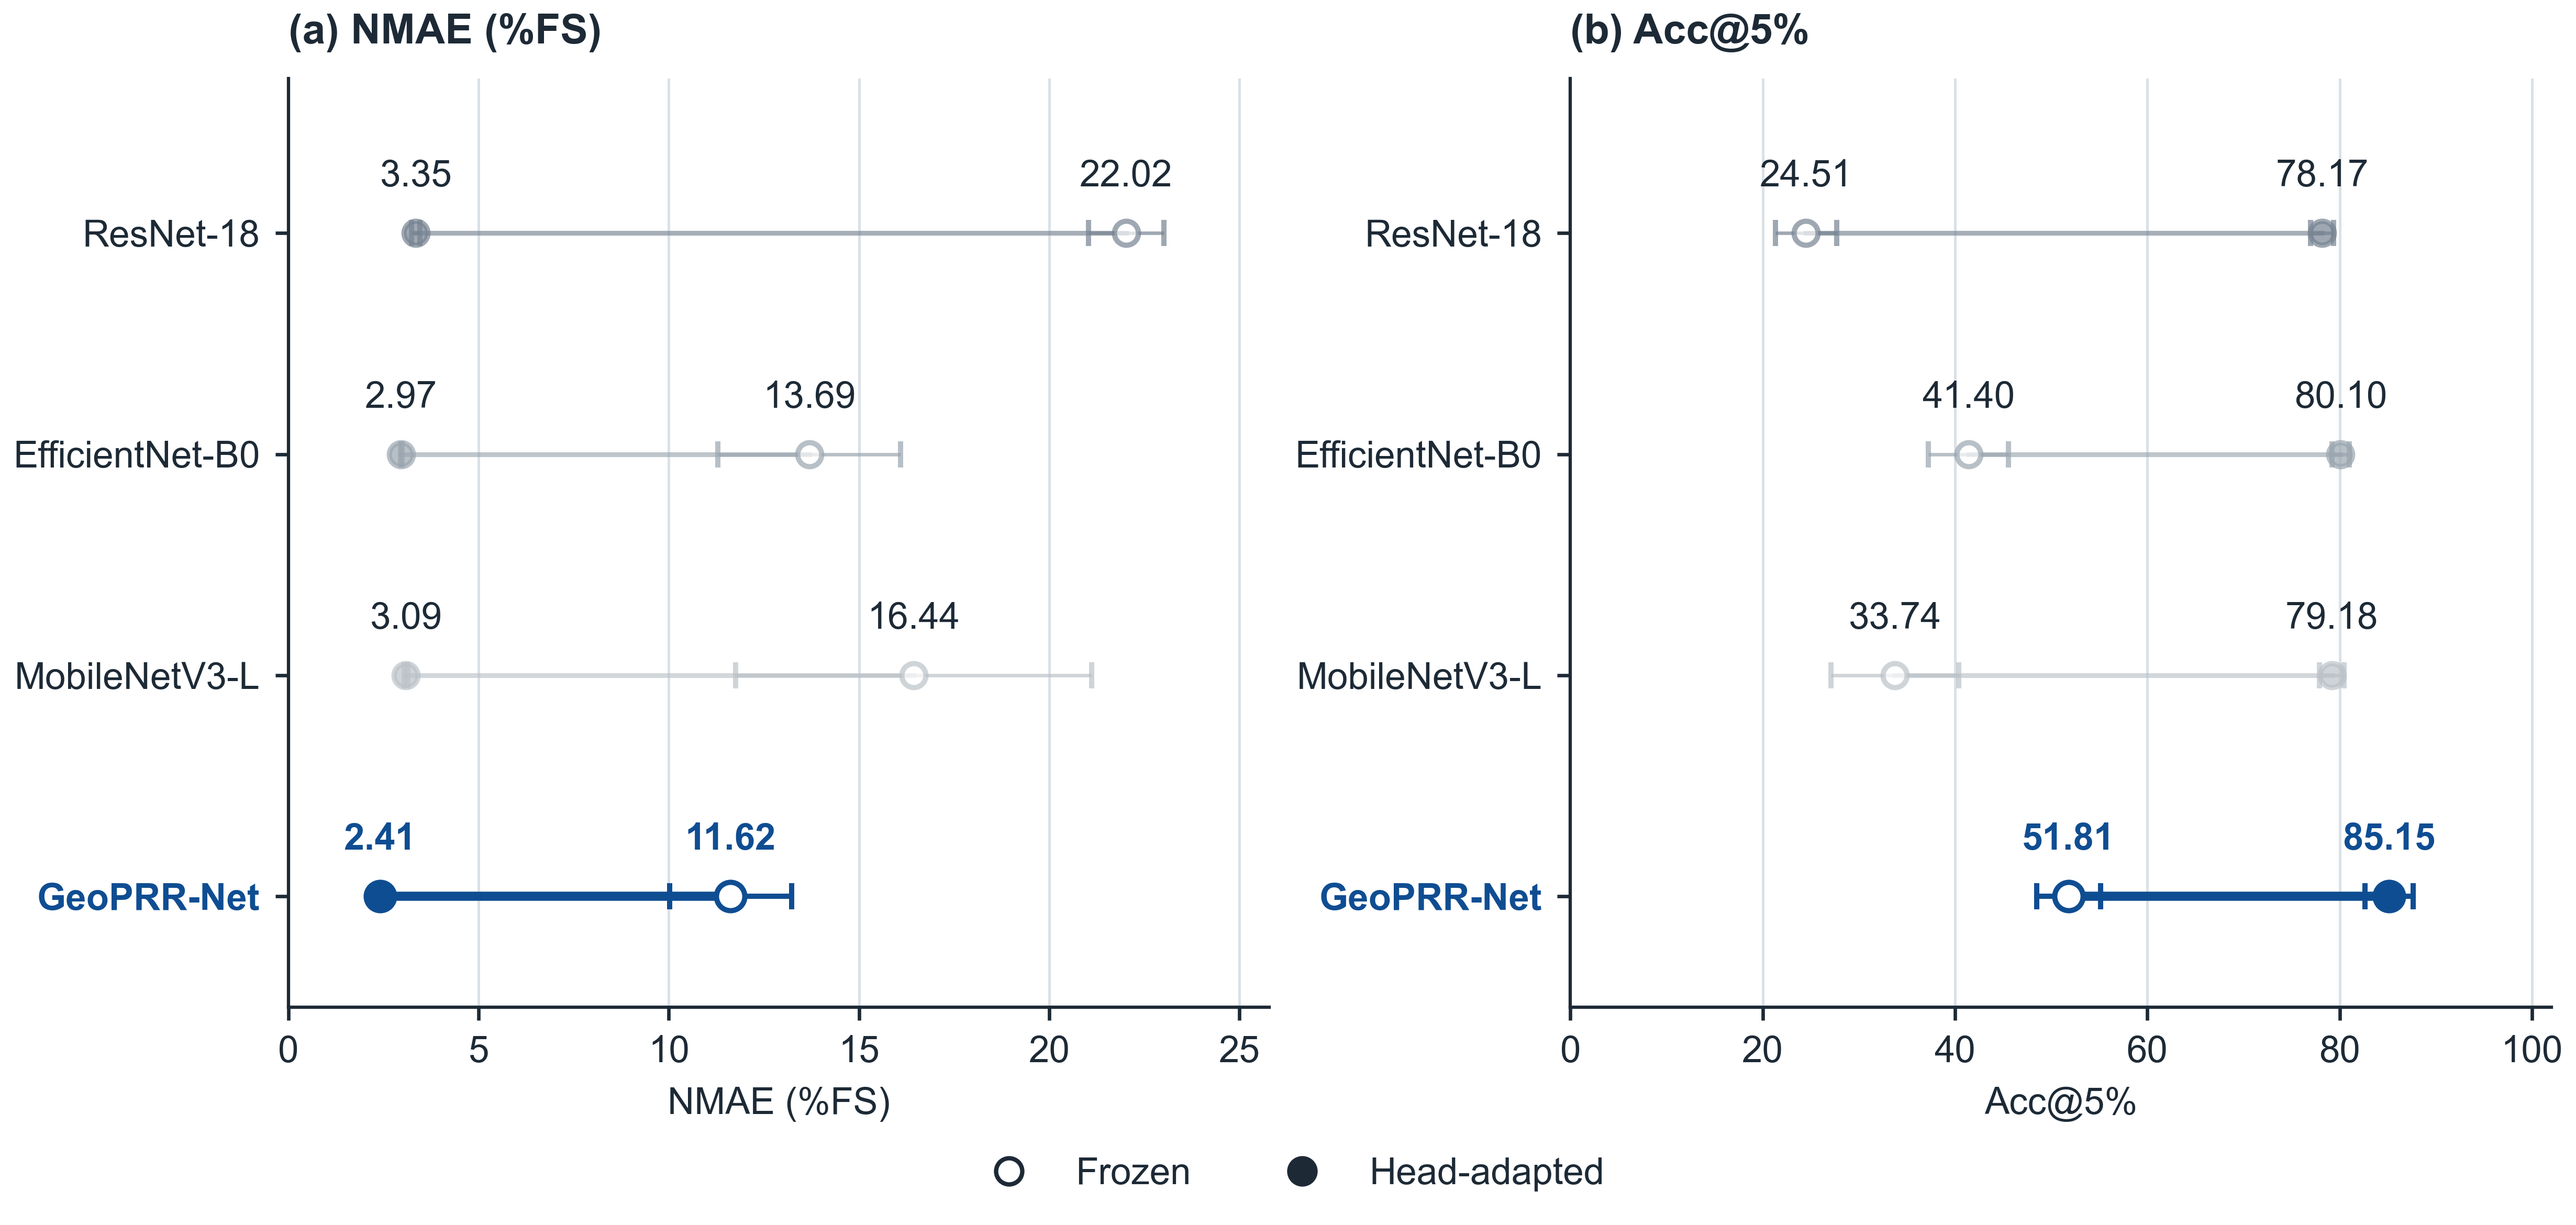
\includegraphics[width=\textwidth]{fig4_industrial_1395.png}
\caption{Frozen-source and retained readout-head-adapted results on Industrial-1395. (\textbf{a}) NMAE in \%FS. (\textbf{b}) Acc@5\% in percent. Each row compares predictions on the same complete six-condition roster. Points and whiskers show means and sample standard deviations over the three source seeds, and connecting lines link the two reported settings. \modelname is highlighted in blue and uses the two source configurations defined in Table~\ref{tab:industrial}; raw CNNs retain matched before--after controls. Source feature extractors were frozen during the retained adaptation experiments. Three-member ensemble results are listed separately in Table~\ref{tab:industrial}.}
\label{fig:industrial}
\end{figure}

\subsection{Geometry, Routing, and Relational-Transport Ablations}
\label{subsec:mechanisms}
\label{subsec:ablation_results}
\label{subsec:routing_results}

Table~\ref{tab:ablation_results} compares the updated full model with the three retained variants. The largest pooled NMAE gap was associated with the no-geometry variant, followed by the fixed mixture and no-relational variant; all three variant-minus-full intervals were above zero. Figure~\ref{fig:ablation_routing}(\textbf{c}) locates much of this separation in the projective conditions. For example, the no-geometry gap increased from 0.0849\%FS on clean inputs to 1.4319\%FS under combined severe distortion, whereas the clean and blur gaps were much smaller. The fixed-mixture and no-relational variants showed the same broad concentration of differences under perspective perturbation. This condition dependence connects the configuration comparison to the geometric robustness problem that motivates the method.

\begin{table}[H]
\caption{Retained core variants compared with the updated full model on the complete SyncG test roster. Values are mean $\pm$ sample SD over three seeds. NMAE and variant-minus-full differences are in \%FS; Acc@5\% is in percent. Intervals use 20,000 paired scene-group bootstrap replicates after averaging errors across seeds. Full uses the updated full-source fit; variant measurements retain the original fitting protocol described in Section~\ref{subsec:ablation_protocol}.}
\label{tab:ablation_results}
\centering
\small
\begin{tabularx}{\textwidth}{@{}>{\raggedright\arraybackslash}Xccc@{}}
\toprule
\textbf{Variant} & \textbf{NMAE $\downarrow$} & \textbf{Acc@5\% $\uparrow$} & \textbf{Difference [95\% CI]} \\
\midrule

Full model & $0.7407\pm0.0220$ & $98.90\pm0.04$ & --- \\

Without geometry-aware fusion & $1.3452\pm0.0327$ & $96.38\pm0.22$ & $0.6045$ [$0.5742,0.6367$] \\

Fixed expert mixture & $1.0104\pm0.0299$ & $97.86\pm0.24$ & $0.2697$ [$0.2491,0.2920$] \\

Without relational transport & $0.9210\pm0.0384$ & $98.41\pm0.29$ & $0.1803$ [$0.1643,0.1977$] \\

\bottomrule
\end{tabularx}
\end{table}

Figure~\ref{fig:ablation_routing}(\textbf{a}) organizes the four configuration-level operating points. Lower NMAE was observed at the dynamic-routing point in both geometry settings. The displayed geometry-by-routing contrast is $-0.1411$\%FS (95\% CI $[-0.1600,-0.1236]$\%FS). It combines the updated geometry-on/dynamic full-model cell with the three retained fixed-routing or geometry-off cells. Read together with the condition-wise gaps, this plot identifies viewpoint robustness as the main setting in which the tested configurations separate.

\begin{figure}[H]
\centering
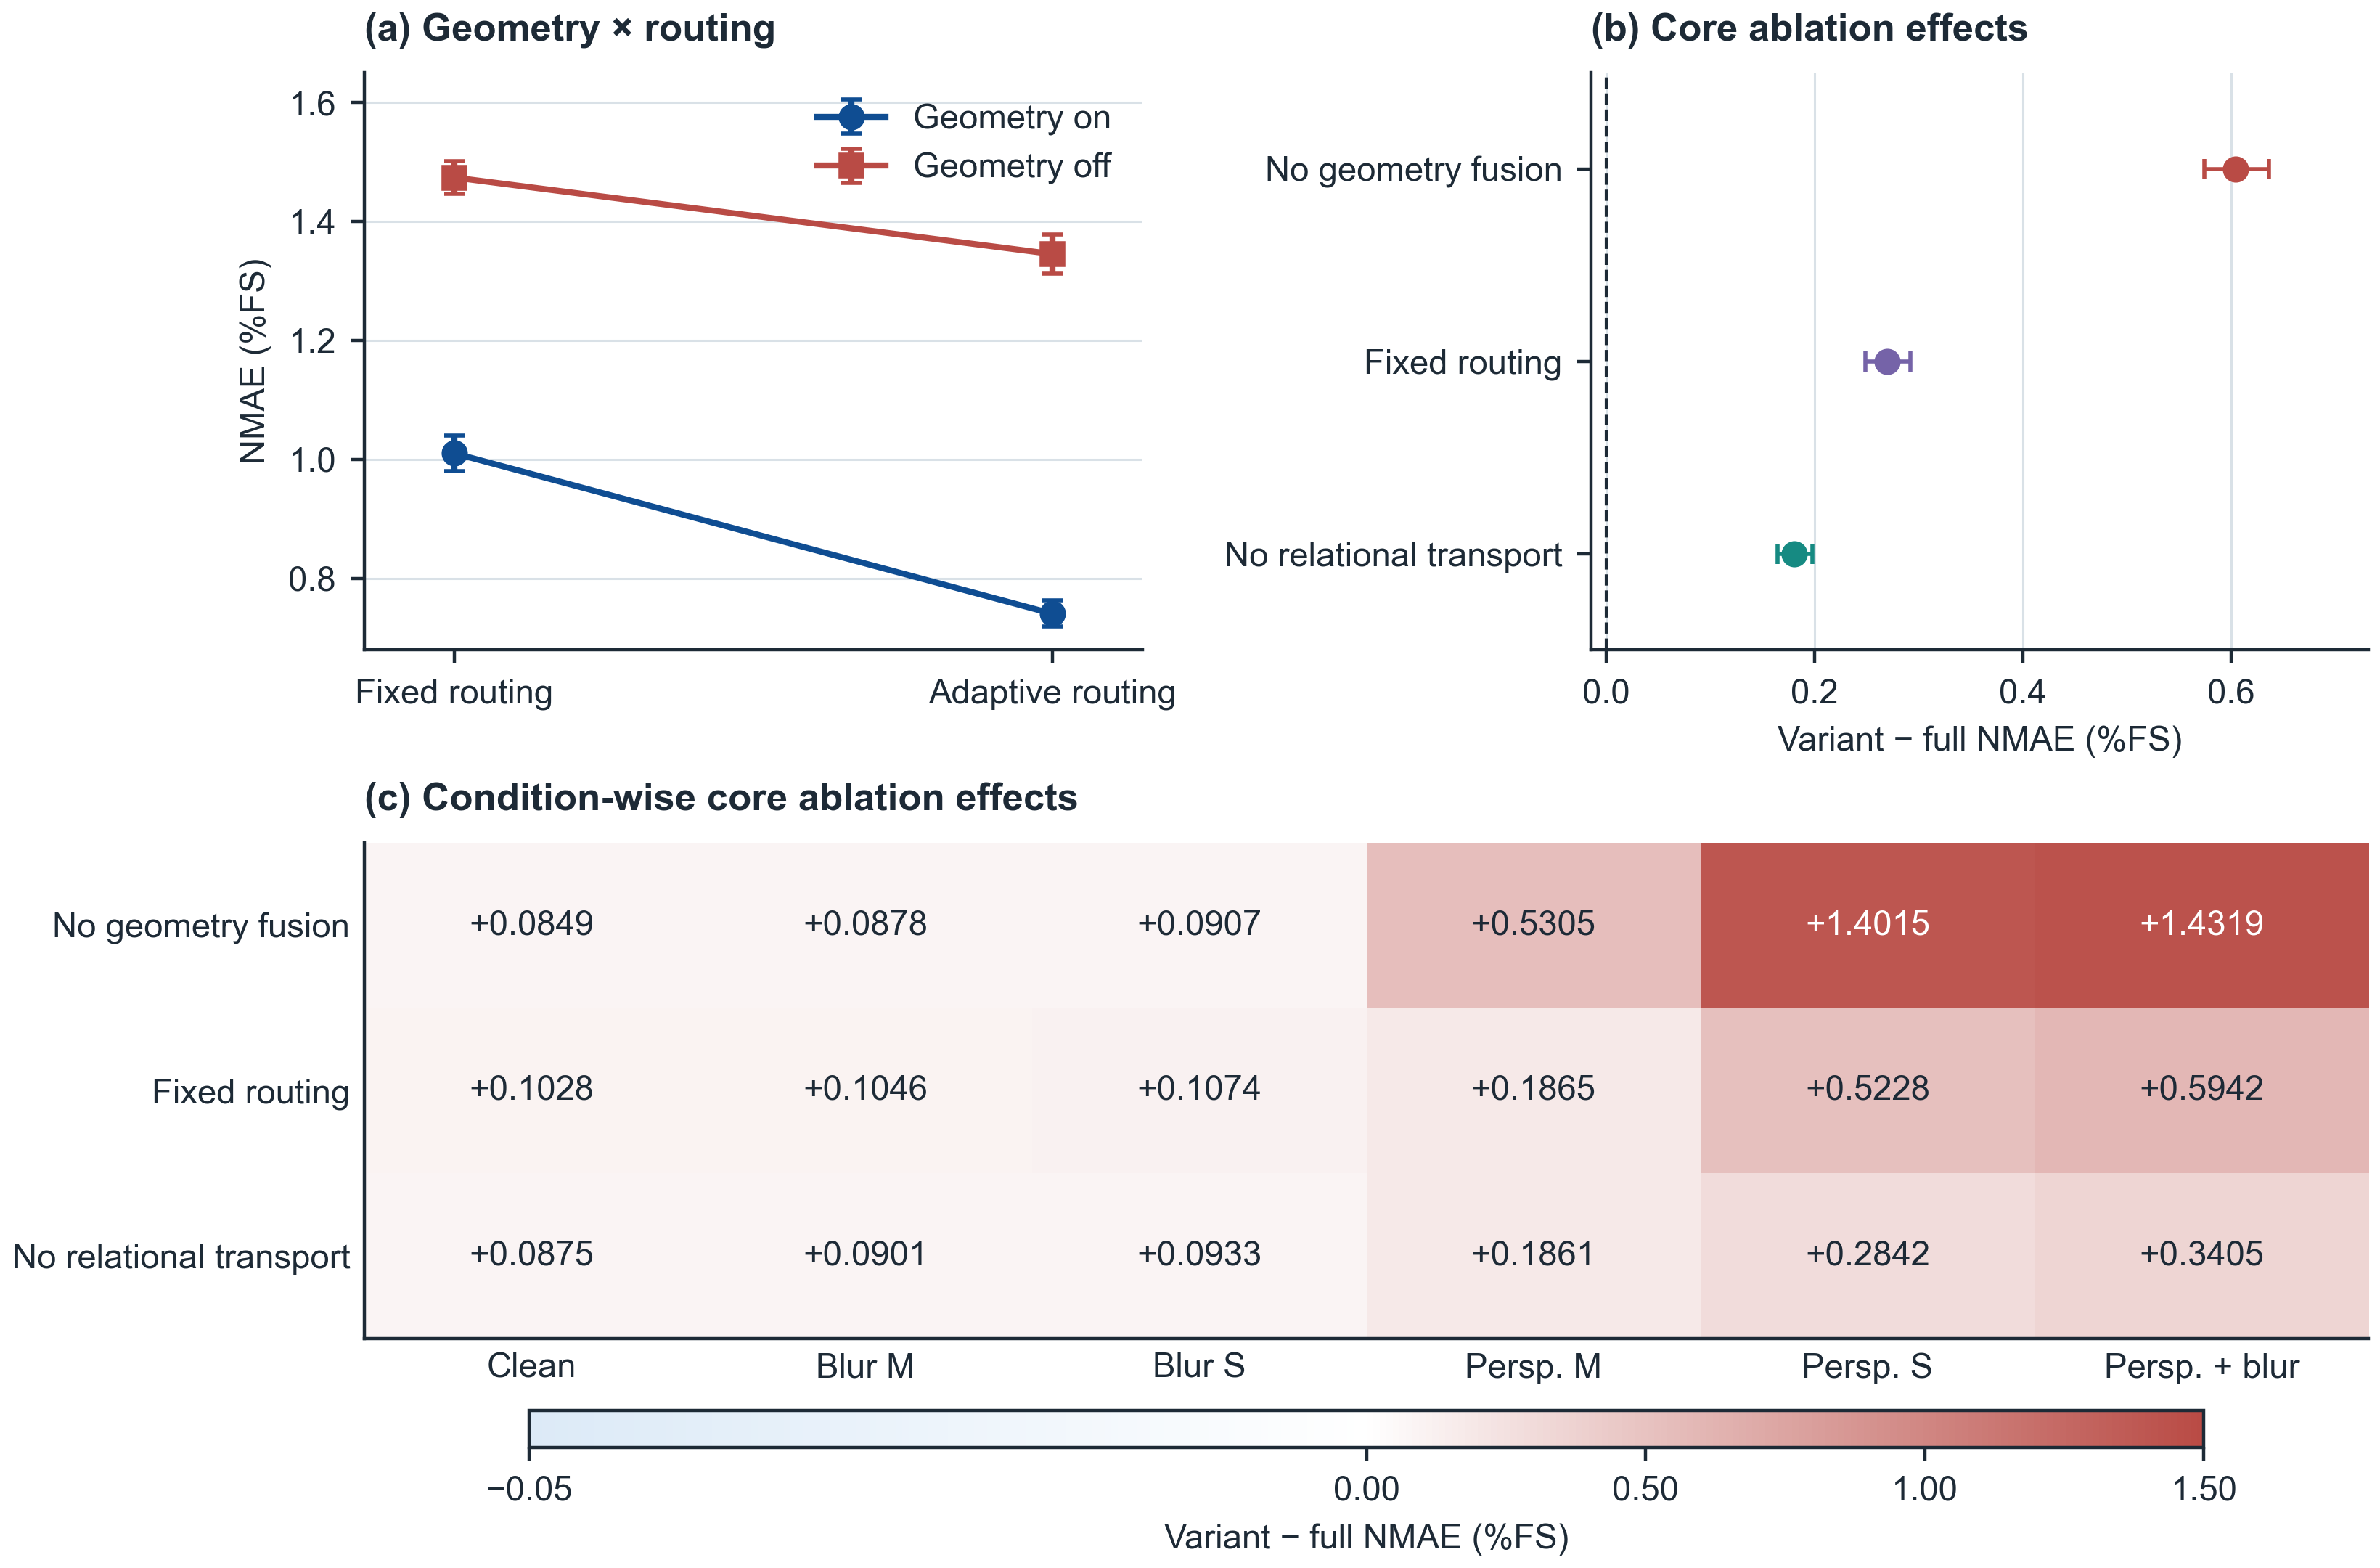
\includegraphics[width=\textwidth]{fig3_ablation_routing.png}
\caption{Retained variants and the updated full model on SyncG. (\textbf{a}) The $2\times2$ geometry-by-routing comparison, reported as NMAE mean and sample SD over three seeds. The geometry-on/dynamic cell is the updated full model; the other cells retain their original fits. The displayed contrast is $(\mathrm{geometry\ on,dynamic}-\mathrm{geometry\ on,fixed})-(\mathrm{geometry\ off,dynamic}-\mathrm{geometry\ off,fixed})$. (\textbf{b}) Pooled variant-minus-full NMAE differences for the three retained variants; whiskers are paired 95\% scene-group bootstrap intervals. (\textbf{c}) Mean differences across all six conditions. Model configurations follow Table~\ref{tab:ablation_results}.}
\label{fig:ablation_routing}
\end{figure}

\subsubsection{Routing-Scale Sensitivity}
\label{subsec:alpha_sensitivity}

We varied the routing scale at inference while keeping each trained checkpoint fixed. The tested values were $\alpha\in\{0,10,25,50,100,200\}$, with the prior fixed to $(0.50,0.25,0.25)$. NMAE changes were computed relative to the same dataset and source seed at $\alpha=100$ before aggregating the three paired seed values. The six-condition rosters contained 24,000, 906, and 8,370 rows per seed for SyncG, RF100-VL, and Industrial-1395, respectively. The projective-three subsets comprised moderate perspective, severe perspective, and combined severe distortion, with 12,000, 453, and 4,185 rows per seed. Failed readings remained in the full denominator.

Weight concentration was measured as the percentage of evaluated rows satisfying $\max_k w_k>0.95$. At the default scale, the weights of all three experts were averaged over the six conditions within each seed and then across the same three seeds. Figure~\ref{fig:alpha_prior_sensitivity} reports the paired error changes, weight concentration, and default expert composition. These measurements characterize inference sensitivity for fixed learned weights; the default scale remains $\alpha=100$.

\begin{figure}[H]
\centering
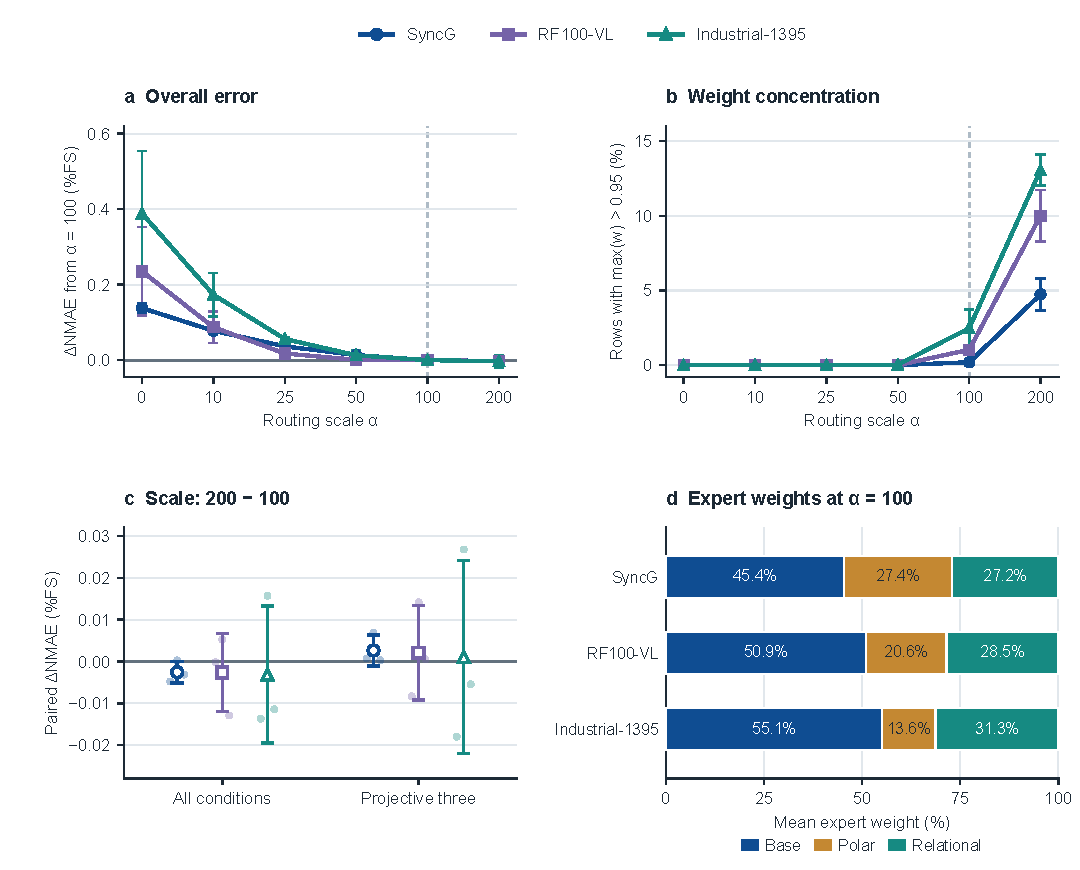
\includegraphics[width=\textwidth]{fig_alpha_prior_sensitivity.pdf}
\caption{Frozen-model routing-scale sensitivity and default expert composition. (\textbf{a}) Six-condition NMAE change relative to the same seed at $\alpha=100$, with the prior fixed to $(0.50,0.25,0.25)$. (\textbf{b}) Percentage of evaluated rows with maximum expert weight greater than 0.95. The six tested scales are displayed at equally spaced positions, with connecting lines used only as visual guides; dashed vertical lines mark $\alpha=100$. (\textbf{c}) Paired NMAE changes from $\alpha=100$ to 200 for the complete six-condition and projective-three rosters. Small points show the individual paired seed differences. Points and error bars in (\textbf{a}--\textbf{c}) show means and sample standard deviations over seeds 20262020, 20262021, and 20262022, not confidence intervals; negative error changes indicate lower NMAE. The reference difference in (\textbf{a}) is zero by construction. (\textbf{d}) Mean base, polar-evidence, and relational-transport weights at $\alpha=100$, averaged within each seed over all six conditions and then across seeds. Labels are percentages rounded to one decimal place; component SD bars are not placed on cumulative stack boundaries. Colors identify datasets in (\textbf{a}--\textbf{c}) and experts in the local legend of (\textbf{d}).}
\label{fig:alpha_prior_sensitivity}
\end{figure}

The retained fixed-model inference sweep supports $\alpha=100$ as a useful balance between reading error and expert allocation. Overall NMAE reductions largely levelled off around this setting. Increasing the scale to 200 produced only marginal decreases in three-seed mean NMAE over the six-condition rosters, while slightly increasing the projective-three mean errors and concentrating the expert weights across all three datasets. The default therefore preserved nearly the same pooled error as the larger scale with less concentrated allocation and slightly lower mean errors on the projective subsets. Panel (\textbf{d}) further shows that mean expert allocation changes across cohorts, consistent with conditional use of the available evidence. Together, these observations give a practical rationale for the default on the examined fixed checkpoints.

\subsection{Accuracy and Complete-Reader Efficiency}
\label{subsec:efficiency_results}

Table~\ref{tab:efficiency} reports complete frozen ROI-to-reading pipelines under the batch-1 FP32 protocol in Section~\ref{subsec:efficiency_protocol}. Figure~\ref{fig:reader_tradeoff} highlights the compact parameter and memory footprint associated with the proposed reader's accuracy. \modelname uses fewer parameters and less peak allocated memory than all three structured readers, while its updated Industrial-1395 NMAE is lower. This combination is useful when numerical reading quality and memory requirements are important design considerations. Its recorded P50 latency is 47.895~ms and its throughput is 20.29 ROIs/s, making it the slowest of the seven measured pipelines; the P50-to-P95 span also shows execution-time variation beyond the median. The updated accuracy and retained execution measurements therefore expose the complete reading-error and runtime trade-off, which parameter counts alone cannot express.

\begin{table}[H]
\caption{Complete-reader efficiency for seven frozen methods with 20 warm-up and 100 timed calls. Latency includes ROI preprocessing, transfers, networks, and conversion to a reading; file decoding and labels are excluded. VDN and DeepLab include the source-trained pose reference detector. \modelname uses one source checkpoint. Peak memory is allocated CUDA memory in MiB. Accuracy uses the complete Industrial-1395 roster, whereas timing follows the 100-call protocol in Section~\ref{subsec:efficiency_protocol}.}
\label{tab:efficiency}
\centering
\small
\begin{tabularx}{\textwidth}{@{}>{\raggedright\arraybackslash}Xccccc@{}}
\toprule
\textbf{Method} & \textbf{Params (M)} & \textbf{P50 (ms)} & \textbf{P95 (ms)} & \textbf{ROIs/s} & \textbf{Peak MiB} \\
\midrule

Raw ResNet-18 & 11.177 & 2.725 & 3.840 & 346.17 & 78.2 \\

Raw EfficientNet-B0 & 4.009 & 5.130 & 6.356 & 190.19 & 37.4 \\

Raw MobileNetV3-Large & 4.203 & 4.544 & 5.904 & 208.66 & 56.4 \\

YOLO11s-Pose-4KP & 9.700 & 6.227 & 7.934 & 152.58 & 84.3 \\

VDN & 25.077 & 13.758 & 16.445 & 70.69 & 158.2 \\

DeepLabV3+-ROI & 50.047 & 30.662 & 33.807 & 32.30 & 306.5 \\

\modelname & 4.885 & 47.895 & 62.087 & 20.29 & 43.4 \\

\bottomrule
\end{tabularx}
\end{table}

\begin{figure}[H]
\centering
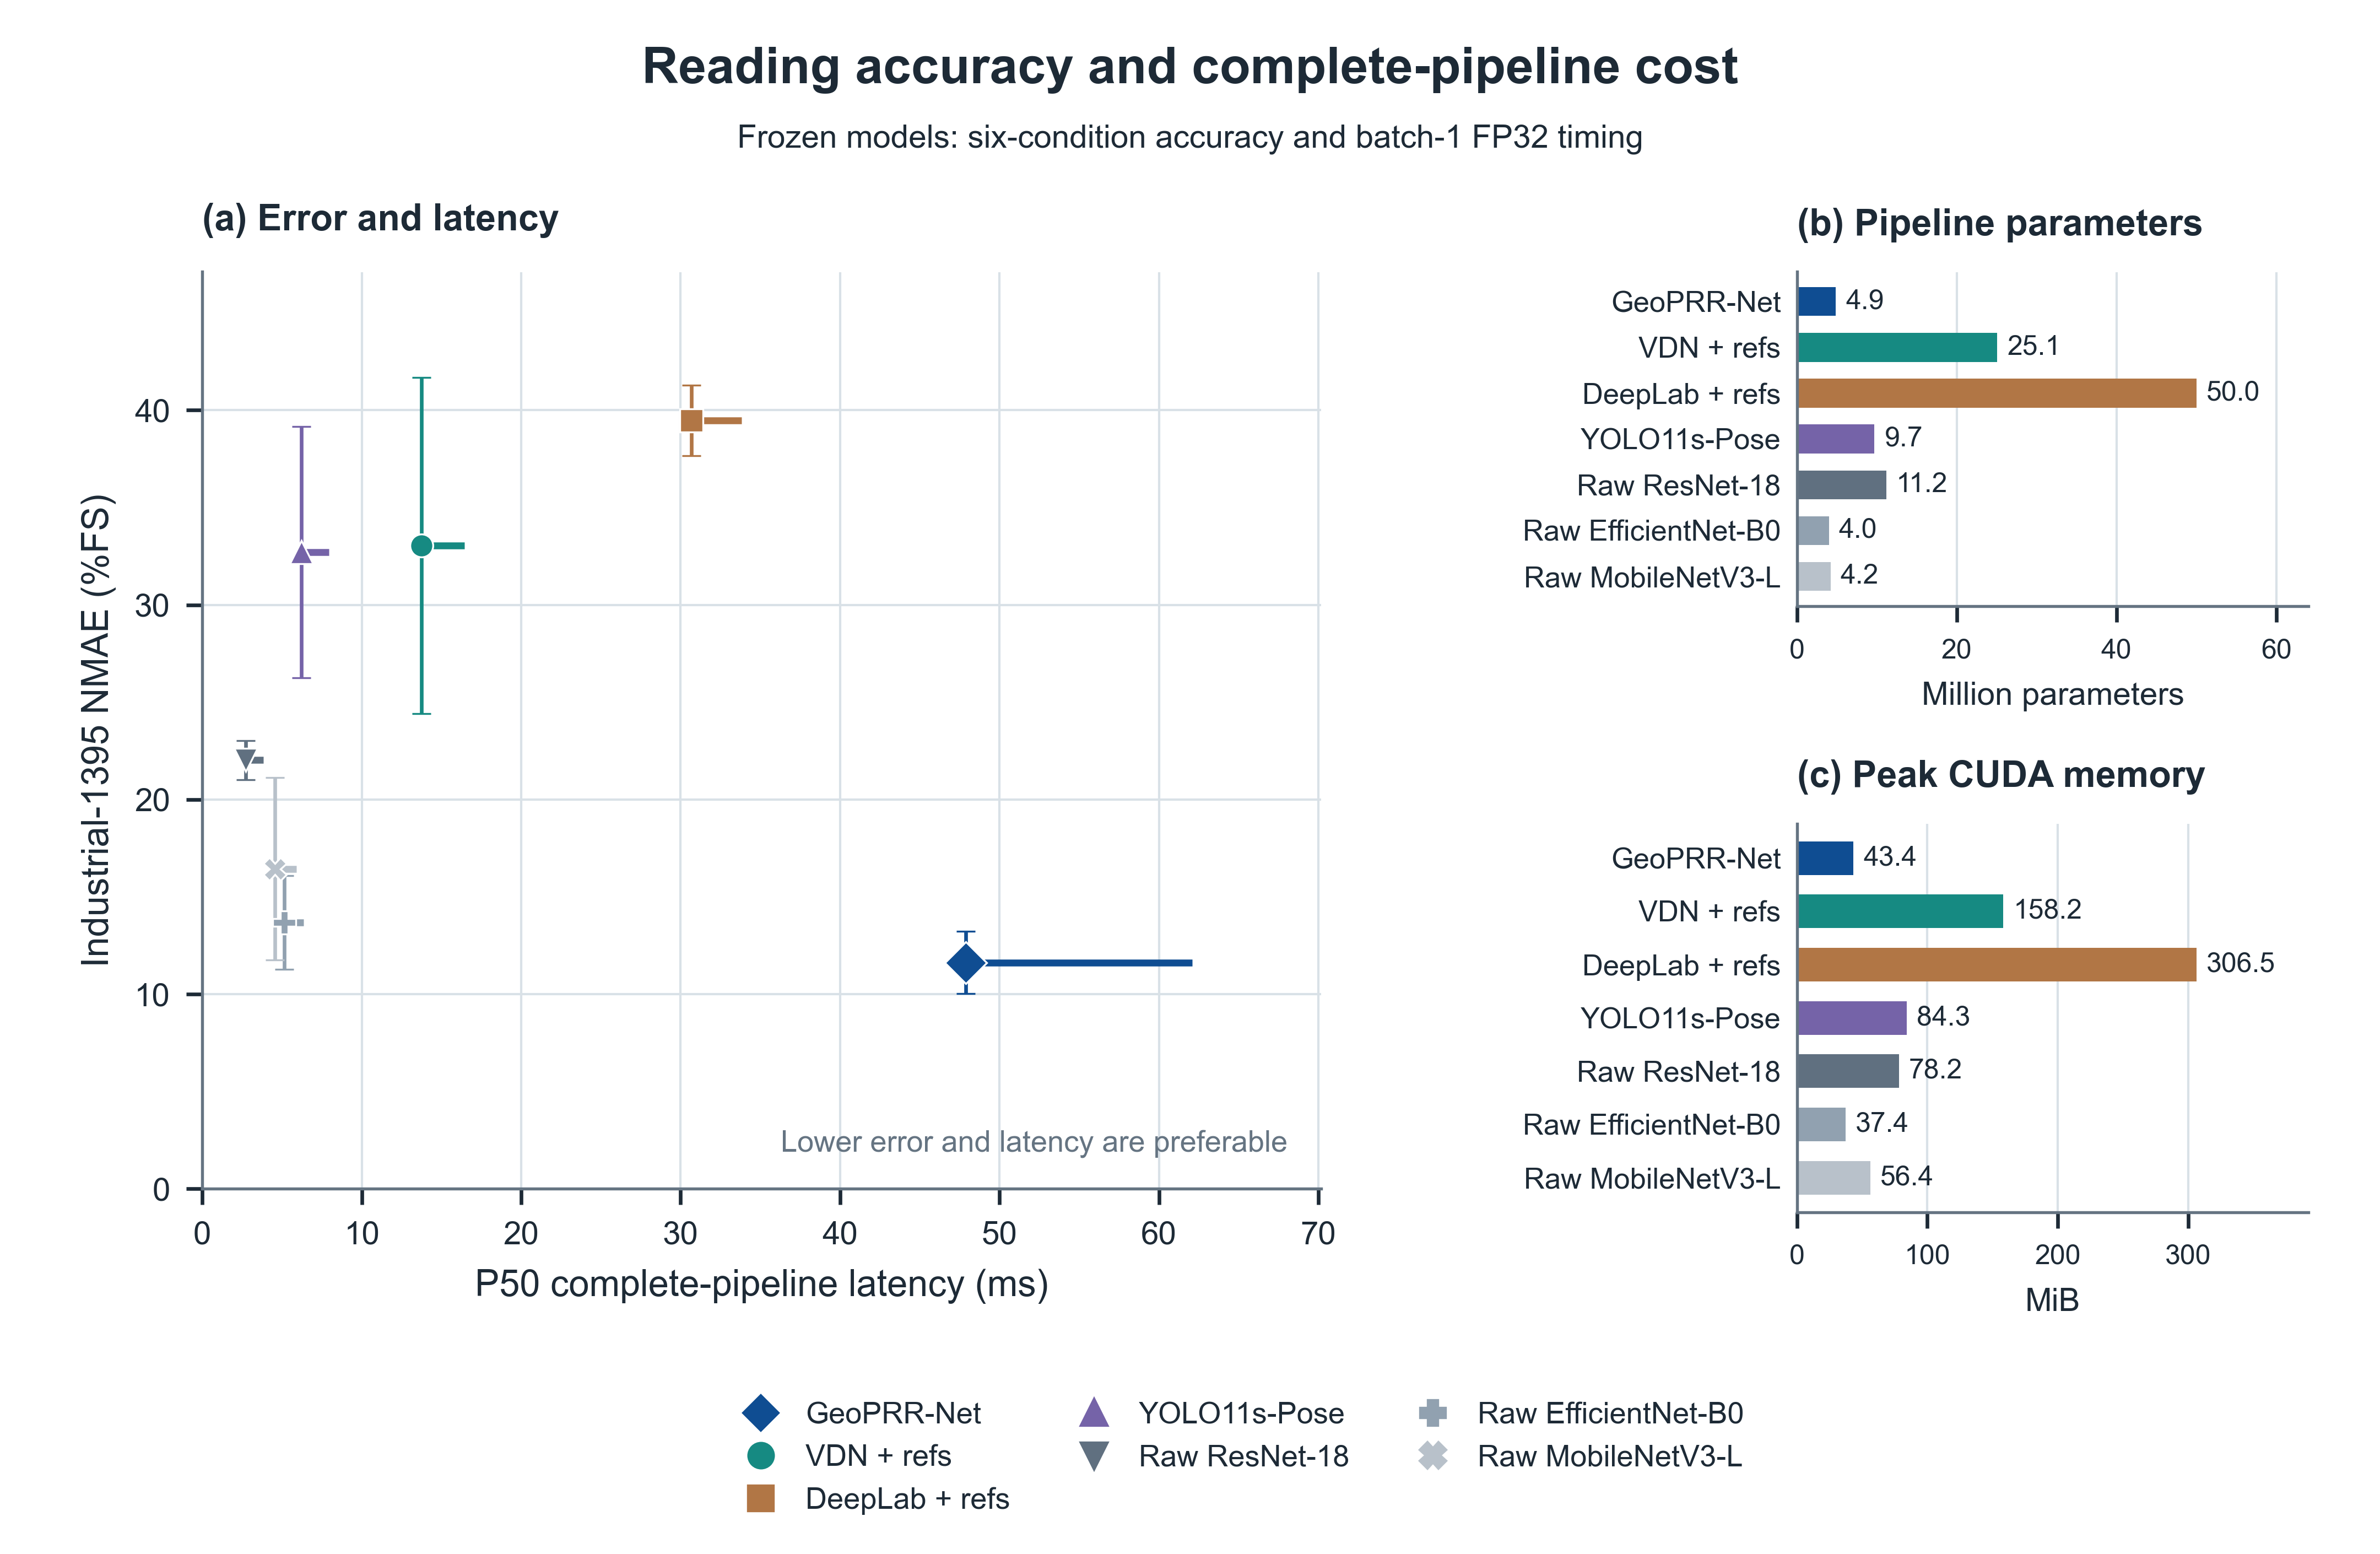
\includegraphics[width=\textwidth]{fig_complete_reader_tradeoff.png}
\caption{Accuracy and complete-pipeline costs for the seven frozen readers. (\textbf{a}) Industrial-1395 six-condition NMAE versus P50 batch-1 FP32 latency. Vertical bars are the NMAE sample SD across three seeds; horizontal segments run from P50 to P95 latency and are not confidence intervals. (\textbf{b}) Parameter counts for the complete pipelines. (\textbf{c}) Peak allocated CUDA memory. VDN and DeepLab include their automatic reference detector. Adapted models and ensembles are excluded from these frozen comparisons.}
\label{fig:reader_tradeoff}
\end{figure}

For the supervised setting, Table~\ref{tab:adapted_efficiency} compares one adapted member with the corresponding three-member ensemble for each method. The retained adapted ensembles improve reading accuracy, but they also increase complete-reader latency and peak memory. Their benefit must therefore be assessed against the required reading rate and the cost of executing additional members. Comparing an ensemble with a single model without retaining this distinction would obscure the execution cost of the higher-accuracy operating point.

\begin{table}[H]
\caption{Matched adapted-reader execution costs under the same batch-1 FP32 timing protocol. Single-member readers include one frozen source encoder and its fitted head; ensembles include all three members and equal-weight prediction averaging. P50 latency is in ms and peak allocated CUDA memory is in MiB.}
\label{tab:adapted_efficiency}
\centering
\small
\begin{tabularx}{\textwidth}{@{}>{\raggedright\arraybackslash}Xcccc@{}}
\toprule
\textbf{Method} & \shortstack{\textbf{Single}\\\textbf{P50}} & \shortstack{\textbf{Ensemble}\\\textbf{P50}} & \shortstack{\textbf{Single}\\\textbf{MiB}} & \shortstack{\textbf{Ensemble}\\\textbf{MiB}} \\
\midrule

Raw ResNet-18 & 3.171 & 10.094 & 79.5 & 168.1 \\

Raw EfficientNet-B0 & 5.785 & 17.800 & 39.1 & 71.5 \\

Raw MobileNetV3-Large & 5.106 & 15.996 & 56.9 & 90.3 \\

\modelname & 47.087 & 154.036 & 44.7 & 85.2 \\

\bottomrule
\end{tabularx}
\end{table}


\section{Discussion}
\label{sec:discussion}

\subsection{Geometry, Relations, and Conditional Allocation}

The central advantage of the proposed reader is preserving numerical reading accuracy when the viewing geometry changes. The paired SyncG comparisons show limited error growth under perspective perturbation together with substantially more recovered than lost tolerance-qualified readings. The retained variant comparisons further concentrate the largest performance gaps in the projective conditions, linking the observed advantages to the geometric problem that motivates the method. The design builds on rectification, keypoint, and scale-structure approaches \cite{bao2019ipm,wang2022scalemark,tan2024transunet,lee2026p2yolo}, while retaining both raw and support-normalized observations for fusion. Access to both observations gives the reader alternative image evidence when the normalized view is less informative, offering a plausible explanation for the observed robustness pattern.

Conditional allocation adds flexibility to how the available candidate estimates are combined. The retained routing-scale sweep supports a setting that maintains low pooled error without forcing strongly concentrated expert weights, while the cohort-level compositions show different mean allocations for different image populations. This is consistent with using heterogeneous evidence according to the input rather than assigning the same effective balance everywhere. The moment projection preserves agreement between the combined estimate and the reported posterior mean as that allocation changes. Together, these properties provide a coherent reading output while allowing the contribution of each evidence path to vary with the observations.

\subsection{Industrial-Electronics Interpretation}

The real-image results show that the learned reading capability transfers beyond the synthetic source cohort. The updated source-trained model led the tested readers in both NMAE and Acc@5\% on RF100-VL and Industrial-1395. The paired outcomes and broad coverage of group-level gains further support that advantage across varied evaluated inputs. This provides evidence for a reusable ROI-level reading component that combines image-derived geometry with learned visual features across the two target cohorts.

A second practical advantage is the ability to obtain strong target-domain performance from frozen source representations with a compact fitted readout. The retained matched experiments show that this strategy benefits several feature extractors and that the original GeoPRR representation retains an accuracy advantage when the CNN controls receive the same head-fitting opportunity. High single-member accuracy and the additional gain from the adapted ensemble provide different operating choices. These findings support separating source feature extraction from target readout fitting when developing readers for a particular instrument population.

The proposed reader also combines its accuracy with a smaller parameter inventory and lower measured peak memory than the structured-reading comparators. These resource characteristics are useful for assessing the memory demands of an implementation. Reading accuracy, coverage, and execution time then provide complementary criteria for selecting an operating point, with ensemble size treated as part of the configuration. The complete ROI-to-reading benchmark makes that decision more informative than a comparison based only on network size. Full-frame localization, asset-range recognition, and data acquisition are additional components to consider when integrating this reading core into an inspection system.

\subsection{Limitations and Future Work}

Zero-shot reading accuracy in real industrial scenes remains an area for improvement. Although \modelname outperforms the comparison methods on both real-image cohorts, many readings on Industrial-1395 still exceed the specified tolerance, indicating that consistently accurate transfer across different instrument populations remains unresolved. Another limitation is prediction reliability: the current model enforces consistency between the reading and the posterior mean but lacks a validated strategy for confidence calibration and abstention. Improving target-domain reading accuracy and enabling the model to identify predictions that require review are therefore priorities for future work.

Execution efficiency also requires further improvement. The recorded implementation has a relatively small parameter inventory and memory footprint compared with the structured readers, but its complete-reader latency remains comparatively high. This may constrain its use in higher-throughput settings. Future work can use operator-level profiling to identify the main execution costs and investigate computational reuse and optimization of the execution path, with the aim of increasing processing speed while preserving reading accuracy.

\section{Conclusions}
\label{sec:conclusion}

This paper presented \modelname, a shared-encoder gauge reader that combines geometry-aware fusion, relational moment transport, and conditional allocation of candidate means. A moment-consistent information projection returns one posterior coherent with the normalized reading. On the official SyncG test split, NMAE is $0.7407\pm0.0220$\%FS compared with $1.6595\pm0.0627$\%FS for Raw EfficientNet-B0. Frozen Industrial transfer and the retained target-supervised experiment provide complementary evidence: relative NMAE reductions are 15.1\% for the updated frozen model, 18.9\% after matched OOF fitting of the original configuration, and 19.3\% for its matched three-member ensembles. Dataset-ordered comparisons with raw CNN and structured-reading baselines, together with the retained variant comparisons, characterize the proposed approach within the evaluated ROI-level setting.

%%%%%%%%%%%%%%%%%%%%%%%%%%%%%%%%%%%%%%%%%%
% MDPI declarations.
\authorcontributions{Conceptualization, X.L.; methodology, X.L.; software, X.L.; validation, X.L.; formal analysis, X.L.; investigation, X.L.; resources, X.L.; data curation, X.L.; writing---original draft preparation, X.L.; writing---review and editing, X.L.; visualization, X.L.; project administration, X.L. The author has read and agreed to the published version of the manuscript.}

\funding{This research received no external funding.}

\institutionalreview{Not applicable. The study evaluates images of instruments and does not involve human participants or animals.}

\informedconsent{Not applicable.}

\dataavailability{SyncG is publicly available at \url{https://doi.org/10.1038/s41597-026-07308-x}, and the RF100-VL gauge subset at \url{https://universe.roboflow.com/rf100-vl/needle-base-tip-min-max-u87vi-wzsrt-kjyu}. Source code is maintained at \url{https://github.com/KongyueX/GeoPRR-Net}. The official full-training experiment's aggregate tables, per-sample normalized targets and predictions, success/failure records, anonymized group statistics, and publication manifest are available in the \texttt{data/official\_syncg\_fulltrain\_20260908} directory of \url{https://github.com/KongyueX/GeoPRR-Net-Paper}. Industrial aliases apply within this release and cannot be joined to similarly numbered identifiers in older packages. Industrial source images, original identities, and physical readings are not redistributed; access is subject to permission from the data owners.}

\acknowledgments{}

\conflictsofinterest{The author declares no conflict of interest.}

\abbreviations{Abbreviations}{%
\begin{tabular}{@{}ll}
CNN & Convolutional neural network\\
FP32 & 32-bit floating point\\
KL & Kullback--Leibler\\
MoE & Mixture of experts\\
NMAE & Normalized mean absolute error\\
OCR & Optical character recognition\\
ROI & Region of interest\\
VDN & Vector Detection Network\\
\end{tabular}}

\appendixtitles{yes}
\appendixstart
\appendix
\section{Supplementary Diagnostics}
\label{app:supplementary_diagnostics}

\subsection{Annotation-Assisted Reference Diagnostics}
\label{app:annotation_diagnostic}
\label{app:annotation}

The annotation-assisted settings provide reference geometry during conversion of the VDN and DeepLab outputs. Table~\ref{tab:annotation_diagnostic} reports these settings separately from the automatic rankings in the main text.

\begin{table}[H]
\caption{Automatic versus annotation-assisted geometric conversion for source-trained VDN and DeepLab. NMAE values are mean $\pm$ sample SD in \%FS over three seeds on the same complete six-condition rosters. The annotation-assisted columns use additional reference information and are diagnostic comparisons, not automatic deployment results.}
\label{tab:annotation_diagnostic}
\centering
\small
\begin{tabularx}{\textwidth}{@{}ll>{\centering\arraybackslash}X>{\centering\arraybackslash}X@{}}
\toprule
\textbf{Dataset} & \textbf{Reader} & \textbf{Automatic NMAE} & \textbf{Assisted NMAE} \\
\midrule

SyncG & VDN & $5.0129\pm2.5266$ & $1.4826\pm0.0662$ \\

SyncG & DeepLabV3+-ROI & $10.2757\pm2.6382$ & $2.9473\pm0.7504$ \\

RF100-VL & VDN & $19.6971\pm6.6315$ & $13.8269\pm3.6075$ \\

RF100-VL & DeepLabV3+-ROI & $30.4040\pm2.6979$ & $23.7993\pm2.5994$ \\

\bottomrule
\end{tabularx}
\end{table}

%%%%%%%%%%%%%%%%%%%%%%%%%%%%%%%%%%%%%%%%%%
\begin{adjustwidth}{-\extralength}{0cm}
\reftitle{References}
\externalbibliography{yes}
\bibliography{references}
\end{adjustwidth}

\end{document}
